% ****** Start of file apssamp.tex ******
%
%   This file is part of the APS files in the REVTeX 4.1 distribution.
%   Version 4.1r of REVTeX, August 2010
%
\documentclass[reprint,%article
 %,
%superscriptaddress,
%groupedaddress,
%unsortedaddress,
%runinaddress,
%frontmatterverbose, 
%preprint,
%showpacs,preprintnumbers,
%nofootinbib,
%nobibnotes,
%bibnotes,
 amsmath,amssymb,
 aps,
%pra,
%prb,
%rmp,
%prstab,
%prstper,
%floatfix,
]{revtex4-1}

\usepackage{xcolor}

\usepackage{graphicx}% Include figure files
\usepackage{dcolumn}% Align table columns on decimal point
\usepackage{bm}% bold math
\usepackage{appendix}
\usepackage{subcaption}
%\usepackage{subfloat}
%\usepackage{hyperref}% add hypertext capabilities
%\usepackage[mathlines]{lineno}% Enable numbering of text and display math
%\linenumbers\relax % Commence numbering lines

%\usepackage[showframe,%Uncomment any one of the following lines to test 
%%scale=0.7, marginratio={1:1, 2:3}, ignoreall,% default settings
%%text={7in,10in},centering,
%%margin=1.5in,
%%total={6.5in,8.75in}, top=1.2in, left=0.9in, includefoot,
%%height=10in,a5paper,hmargin={3cm,0.8in},
%]{geometry}https://www.overleaf.com/project/5ba0361831a91c7b3990c0d7
 \usepackage{natbib}
 
\begin{document}

\preprint{APS/123-QED}

\title{DRAFT- Rotation Curve Fitting Model }% Force line breaks with \\
%\thanks{ Thanks Jesus}%

% Find out if Joe and Noah still want to be on this paper%

 

\author{Sophia Natalia Cisneros}
 \affiliation{ Department of Astronomy,  
 University of Washington}
 % \email{sophia.cisneros@du.edu}
  \author{Richard Ott}%
 \email{rich.ott@EMAIL.com}
\affiliation{Affiliate MIT - Ask Joe Formaggio}%Tech dudes \textbackslash\textbackslash
%}
 \author{ Meagan Crowley}
\email{ }
\affiliation{NREL}%
 \author{ Amy Roberts}
\email{ }
\affiliation{CU Denver}%
\author{Marcus Paz}
\author{Zaneeyiah Brown}
\author{Landon Joyal}
\author{Roberto Real Rico}
\author{Elizabeth Gutierrez-Gutierrez}
\author{ Phong Pham}
\author{Zac Holland}
\author{Amanda Livingston}
\author{Lily Castrellon}
\author{Shanon Rubin}
\author{Aaron Ashley}
\author{Dillon Battaglia}
%\affiliation{UMass Boston% with \\
%&}%
%
 
 
\date{\today}% It is always \today, today,
             %  but any date may be explicitly specified
             %%%%%%
%%%%%%%
%%%%%%
%%%%%%%
%%%%%%
%%%%%%%
\begin{abstract}
 
 
{\color{teal}   Github repo: Cisneros-Galaxy/RCFM     }

\begin{description}
\item[Usage]
Secondary publications and information retrieval purposes.
\item[PACS numbers]
May be entered using the \verb+\pacs{#1}+ command.
%\item[Structure]
%You may use the \texttt{description} environment to structure your abstract;
%use the optional argument of the \verb+\item+ command to give the category of each item. 
\end{description}
\end{abstract}

\pacs{Valid PACS appear here}% PACS, the Physics and Astronomy
                             % Classification Scheme.
%\keywords{Suggested keywords}%Use showkeys class option if keyword
                              %display desired
\maketitle

%\tableofcontents
%%%%%%NOTES TO DO
%%%make labels for figure axes. remove orange line through the data
%%%%%%
%%%%%%%%
%%%%%%
%%%%%%%
%%%%%%
%%%%%%
\section{Introduction  \label{sec:uno}}


%DARK MATTER

 The flat-rotation curve problem of spiral galaxies  is viewed as primary evidence for dark matter\cite{Rub,Bosma,1985ApJAlbada}. 
 In the dark matter paradigm, this problem is   viewed as a missing mass component due to a conflict between kinematic phrasing of  two      observations of light, spectra and photometry. Photometry yields Keplerian orbital velocities, which fall-off outside of the stellar light. Doppler shifted spectra yields rotation velocities from the Lorentz Doppler shift formula, which do not fall-off outside the stars  (see Fig.~\ref{fig:NGC2403}).  
 
 
 
Dark matter theories are built from classical gravity, but with massive
   ``dark'' particles  which do not interact electromagnetically.   These particles have   yet to be    discovered, but are hypothesized to have a very low interaction probability with baryonic matter, and so  experiments are ever increasing their sensitivity to detect them \cite{Cebrian:2022brv}. In the absence of a direct detection, the paradoxes of dark matter models are interesting. The first paradox is best stated by 
  S. McGaugh  when they ask   ``Why is the luminous tail wagging the dark matter dog,  if dark matter dominates dynamics ?'' \cite{1999McGaugh,McGaugh2016RAR}. This is known as the  disk-halo conspiracy, and means that 
that knowledge of 
 the luminous stellar   disk  completely determine the spherical dark matter halo \cite{2004ApJ...609..652M}.
 
 
 
 A second paradox  is known as  the Universal Rotation Curve(URC)  \cite{salucci,Persic,1978Rubin,10.1111/j.1365-2966.2007.11696.x}, in which  a spectrum of 1,100 galaxy rotation curves
 inflect  about  the Milky Way's assumed  position on the same graph    (Fig.~\ref{fig:URC}).  This spectrum requires that 
  small less dense  dwarf galaxies require   proportionally larger dark matter halos than   huge, centrally dense    galaxies. 
  This result requires fine-tuning in dark  matter models, since
  classically mass accretion rates are proportional to total mass \cite{10.1093/mnras/stt2403}.  This reduces their    predictivity   \cite{MCGAUGH2021220}.  We will here interpret these paradoxes here as an indication of  frame-dependent effects   due to our Milky Way. 
   Previously, the role of 
     galaxy curvatures  in this problem  were    obviated 
       by  Galilean subtraction of   gravitational red-shifts at the  large $r$  limit of the data \citep{MTW}. 
      
 
  
  %MOND   
    
  The leading   alternative theory  to dark matter is Modified Newtonian Dynamics (MOND) \cite{Milgrom}, which  proposes    
  that there is  a changing  physical law of gravity    on the vast length scales of galaxies, that the   luminous mass is the only mass, and that luminous mass can be reconciled with observed centripetal accelerations by modifying the acceleration scale on the huge length scalse of galaxies
  \cite{McGaugh_2014}. 
  This approach  is   predictive across a large sample of  rotation curves,   across a broad   range  of galaxy sizes and morphologies \cite{2016Lelli}. 
  MOND uses only   a single free-parameter to represent the acceleration scale changes, and notably,  in fits to  galaxy rotation curves this number is  roughly constant   across   all spiral   galaxies.  \cite{McGaugh2016RAR,2022A&A...664A..40M}. 
  Previous explorations of  extending MOND into the relativistic regime have given rise to a new theories of gravity  \cite{PhysRevD.70.083509,doi:10.1142/S0217751X0703666X}.  We instead
  present an alternative way to envision extending MOND into the relativistic regime, by 
  transitioning the concept of  changing acceleration   to   that of  changing   relative curvature.   
This rephrases  the     MONDian success at fitting galaxies   to a very effective characterization
  of the effect on the  Milky Way's gravitational potential.
   
 
 
 
 
%RCFM  


   
     In this paper we will introduce a new, heuristic technique of  Lorentz-type   transformations     between galaxies to replace dark matter in the standard fitting formula.   These transformations will be  one-to-one in each galactic radius coordinate,   and parametrized with Newtonian gravitational potentials. 
      In this paper we demonstrate the success of this approach by developing a fitting formalism and fitting   a sample of 174 galaxy rotation curves previously fitted by the MOND and dark matter models  \cite{McGaugh2016RAR,2016Lelli}, so that reduced $\chi^2$ values can be directly compared.  
      
   At this time, there are many problems in   the concordance model of   cosmology which are attributed to dark matter \cite{2010dmp..book.....S}, in
 this paper we address only this  one. 
      We propose   that the other places  where dark matter is invoked     require more complicated  physics assumptions 
      %than are presented here; and can be informed by observations of large scale flows 
      \cite{Tully:2014gfa},
      %,    and the ``too'' early   formation of galaxies 
      \cite{Naidu_2022}. 
     % Discrepancies in estimates of the Hubble Flow from supernovae versus from the cosmic microwave background (CITE) and (WHAT"S THE OTHER ISSUE YO). DO I want to include this? 
      
     % MOND      has a fascinating, compact explanation for another dark matter paradox, the  
  % Tully-Fisher relation \cite{1977A&A....54..661T,McGaugh_2000}, but that also is beyond the scope of the current work unfortunately.   
 %In example, the James Webb Space Telescope may have already falsified dark matter driven galaxy formation \cite{2022arXiv221014915H}.
   
   
      
  
 
 
 
This paper  is organized as follows;
{\bf Section \ref{sec:dos}} constructs  the rotation curve  fitting formula, 
{\bf Section \ref{sec:data}}   describes  the data we use, 
 {\bf Section \ref{sec:analysis}}   discusses our results, 
 and  {\bf Section \ref{sec:conclu}}   discusses implications for future tests.   
  
  
 \begin{figure}[h!]
     \centering
     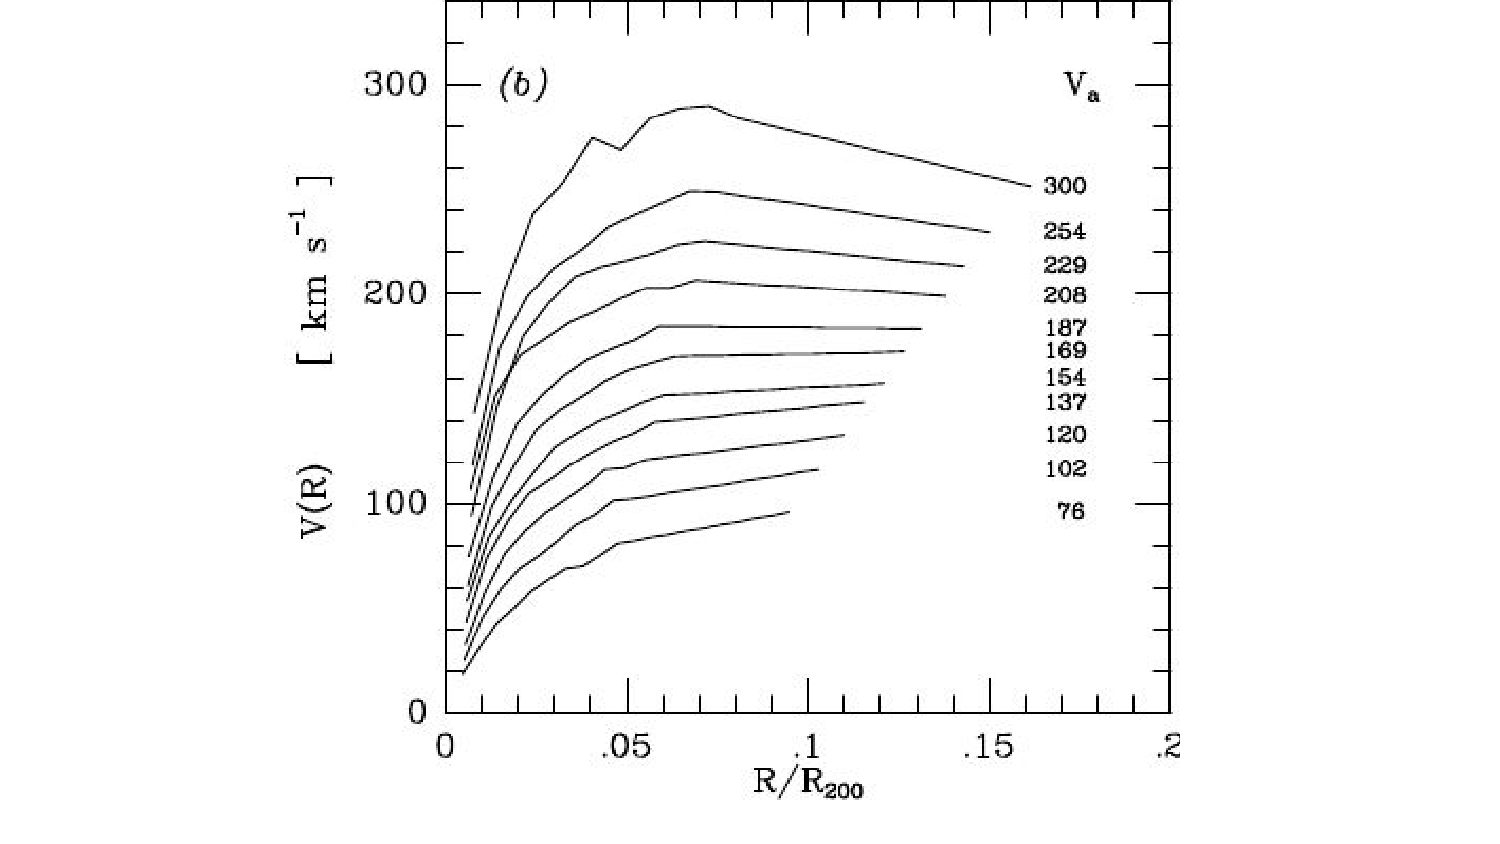
\includegraphics[width=\linewidth]{URC}
     \caption{\emph{Universal Rotation Curve spectrum, Used with permission from Ref.\citep{salucci}}}
     \label{fig:URC}
\end{figure}
  

  
    
 \begin{figure}[h!]
%\scalebox{0.25075}%
      \centering
      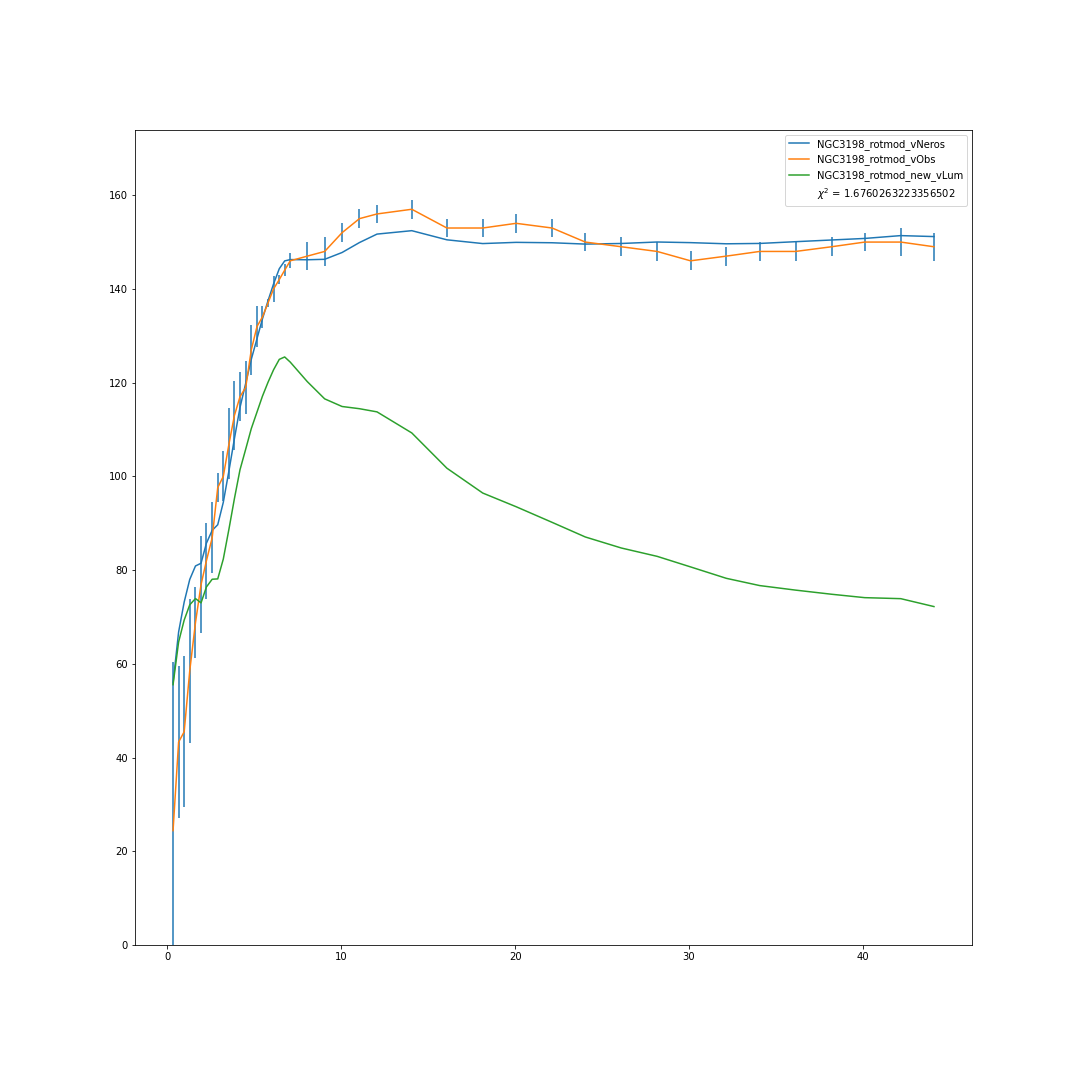
\includegraphics[width=\linewidth]{figures/NGC3198_rotmod_XueSofue.png}
      \caption{\emph{Rotation Curve of NGC 2403 \cite{Blok1}.   Rotation curve data blue dots with  error bars,  Keplerian velocity from luminous mass estimated by   green line,   RCFM fit blue line.} }
      \label{fig:NGC2403}
  \end{figure}
%%%%%%
%%%%%%%%
%%%%%%
%%%%%%%
%%%%%%
%%%%%%
\section{Rotation Curve Fitting Formulae  \label{sec:dos}}
 
{\color{red}NOTE :  Ask Nair   }
{\color{red} \rule{\linewidth}{0.5mm}}
 \subsection{Dark matter rotation curve fitting formula}
 
  

 The   dark matter rotation curve formula   is of the form

 \begin{equation}
v(r)^2_{obs}  =  v(r)^2_{lum}  +  v(r)^2_{dm},   
\label{eq:zonte1}
\end{equation} 

  where all velocities are assumed to be circular orbits about the rotation axis of the galaxy at  $r=0$, in the plane of the galactic disk. 
Terms in  $v_{obs}$ are velocity parameters   from Minkowski spacetime Lorentz boosts 
   

 \begin{equation}
 \frac{v_{obs} }{c}=
\frac{  \left( \frac{\omega'(r)}{\omega_o}\right)^2 -  \left( \frac{\omega_o}{\omega'(r)} \right)^2 }{  \left( \frac{\omega'(r)}{\omega_o}\right)^2  +  \left( \frac{\omega_o}{\omega'(r)}\right)^2 },
\label{eq:modelLumA}
\end{equation} 

 for    
 the rest-frame frequency $\omega_o$, the  observed  Doppler shifted frequency $\omega'$, and $c$  the constant vacuum light speed.  
 Terms in  $v_{lum}$ come from observations of total light  (photometry) interpreted by Population Synthesis Models (PSM) as mass,   hence orbital velocities  
  
   \begin{equation}
v(r)_{lum}^2 = \gamma_b v(r)_{bulge}^2 +  \gamma_d v(r)_{disk}^2 + v(r)_{gas}^2.    
\label{eq:zonte3}
\end{equation} 
  
 Terms in    $\gamma_i$  are the mass-to-light ratios for the stellar bulge $\gamma_b$ and disk $\gamma_d$ respectively, which come from PSM. Gas measurements do not require  a mass-to-light ratio due to different measurement techniques(CITE).  
 Terms in $v^2_{dm}$ represent
the dark matter, and  are  the algebraic difference of the   terms  $v^2_{obs}-v^2_{lum}$. 

  Quadratic terms in  Eq.~\ref{eq:zonte1} and Eq.~\ref{eq:zonte3}  reflect a   sum of gradients in the potential as a function of  radius, 
 for a central gravitational    force law   

\begin{equation}
 \frac{\partial \Phi(r)_{lum}}{\partial r}    =\frac{v(r)_{lum}^2}{r},  
    \label{zoochance1}
\end{equation}

  
   
and a  Newtonian gravitational potential 

\begin{equation}
      \Phi(r)  = -G \int d^3r'  \frac{ \rho(r') }{r-r'} ,
      \label{eq:Newt}
      \end{equation}

which solves Poisson's equation

\begin{equation}
\nabla^2 \Phi(r)_{lum}  = 4\pi G \rho(r).   
    \label{whatsgood}
\end{equation}

 Where $G$ is Newton's   gravitation constant, and 
$\rho(r')$  the mass density. 
  



\subsection{New Rotation Curve Fitting Formula}

  

 

 To test the   new 
frame-dependence picture, 
we  replace the gradient in the potential   attributed to   dark matter      with  Lorentz-type transformations between galaxy frames.   We    assume  luminosity   is a Lorentz scalar, therefore invariant under the assumption of a good distance estimate, and hence a faithful tracer of baryonic mass.  We assume baryonic mass is the only mass in this problem. 
We assume   
   Doppler shifted spectra is part of a Lorentz 4-vector, and so    must transform in a Lorentzian sense.
In addition, we 
   assume   shifts in   spectra   due to relative velocity and relative acceleration are separable \cite{Jack,Cisn}, perhaps roughly  as in Eq.~\ref{eq:zonte1}.
  
   
   
   In what follows, all   terms  can be assumed to  be functions of radius except the model's free parameter $\alpha$,  which is single valued for each galaxy fitted and the speed of light $c$. 
   
   The new rotation curve formula we propose  is
   

\begin{equation}
v_{rc}^2 =  v_{lum}^2+\alpha \kappa^2 v_{1} v_{2},  
\label{eq:zonteLCM}
\end{equation}  

for   a free parameter $\alpha$,  
$\kappa$  a curvature ratio 

 \begin{equation}
\kappa=\frac{\Phi_{gal}}{\Phi_{mw}}, 
\label{eq:kappa2}  
\end{equation}  

 with $\Phi_{gal}$ the    Newtonian gravitational potential of the galaxy being observed, and $\Phi_{mw}$ that of  the Milky Way. 


 Terms in $v_1$   are   
 
   \begin{equation}
       v_1 = \sinh \zeta. 
   \end{equation}
 
 for a rapidity angle $\zeta$ defined by the    Lorentz exponential  term  
  
   
     \begin{equation}
     e^{\zeta}=  \frac{\omega_{mw}}{\omega_{gal}}  =\sqrt{\frac{g_{tt}|_{gal}}{g_{tt}|_{mw}}},
      \label{eq:gravRS}
    \end{equation}
    
 for  clock terms $g_{tt}$   defined in the   weak field Schwarzschild limit  \cite{Hartle}, 
 
  \begin{equation}
      g_{tt}= -( 1 - 2\Phi/ c^2).
      \label{clocktime}
  \end{equation} 
  

Terms in $v_2$ are 

\begin{equation}
v_{2} =  \cosh \tau, 
\label{eq:hyperbolico}
\end{equation}


 
 
  for a rapidity angle $\tau$ defined by the    Lorentz exponential  term  
  
 
\begin{equation}
    e^{\tau}=   e^{(\zeta+\eta)/2},
\end{equation}
 
for the  flat field-frame
Lorentz exponential  

\begin{equation}
    e^{\eta}=\frac{\omega_{l}}{\omega_o}= \sqrt{\frac{1+\beta}{1-\beta}}.   
    \label{eq:flat}
\end{equation}  
     
Terms in 
$\beta = v_{lum}/c$ are the
Keplerian rotation velocities  estimated from total light  $v_{lum}$, and  associated with  frequency shifts $\omega_{l}$      by a Lorentz boost   

 \begin{equation}
 \frac{v_{lum} }{c}=
\frac{  \left( \frac{\omega_{l}}{\omega_o}\right)^2 -  \left( \frac{\omega_o}{\omega_{l}} \right)^2 }{  \left( \frac{\omega_{l}}{\omega_o}\right)^2  +  \left( \frac{\omega_o}{\omega_{l}}\right)^2 }. 
\label{eq:lumlorentz}
\end{equation} 
 
 
  
 
 
The   term $v_1$ maps the gravitational frame of the observed galaxy into that of the Milky Way. The   term $v_2$    maps from  the   curved 2-frame  of  Eq.~\ref{eq:gravRS},  to  the flat 2-frame where we make observations. 
  That this second transformation  is necessary is evidenced by the local constancy of the speed of light. 
  We assert that Keplerian rotation curves are     the best estimate of flatness, since dark matter is not required to  reproduce the rotation curve of our Solar System.
 
    
  
 
  A heuristic construction  and assumptions for integration of the gravitational potentials are described in the next section. Fitting details and analysis are reported in Sec.~\ref{sec:analysis}. 
   
 

 
 
%%%%%%
%%%%%%%
%%%%%%
%%%%%%%  
%%%%%%
%%%%%%%  
\subsection{Gravity Details \label{sec:gravDets}}

%QUESTIONS FOR NAIR
%what is an open ball? 
 % I feel like I"m stating the same thing twice, and maybe not in a consistant way. 
The replacement to dark matter in Eq.~\ref{eq:zonteLCM}, is constructed by  the following heuristic picture. 

We   assume 
   the  additional symmetry of the  Tetrad-formalism \cite{BertschingerClassTetrads}, which attaches  a    local Lorentz frame   at each point in the manifold 


\begin{equation}
    g^{\mu \nu} = \eta^{\alpha \beta} e^\mu_\alpha  e^\nu_\beta
\end{equation} 

so that the orthonormal  basis vectors  $e^\mu_\alpha$ carry the information of the physical spacetime, and the tetrad at each point is Lorentzian and   can endure 3 boosts and 3 rotations \cite{BertschingerClassTetrads}.  
%(ASK CB or NAIR CHECK)
%-  WALD - the basis is the $e^\mu$ and these are $\sqrt{g_{tt}}$ so they not flat, but inner product of one of those bad boys with the inverse covector of the other galaxy, would give us eq. 10, also checkiyo if the indices are correct, originally had a, b lower indices on the basis. CHECK) 
 
   
  Lorentz exponential terms (Eq.~\ref{eq:gravRS} and Eq.~\ref{eq:flat})
  are    identified  as the field frame relationships for the $v_1$ and $v_2$ transformations. We arrive at this result  by  comparison of 
     the  Lorentz transformation in  Eq.~\ref{eq:modelLumA} with 
 that of the    hyperbolic form \cite{rindler2013essential} 


     \begin{equation}
         \frac{v}{c} = \tanh \theta = \frac{e^\theta - e^{-\theta}}{e^\theta + e^{-\theta}} .   
         \label{boost}
     \end{equation} 

 The  $v_1$ and $v_2$ functions reported here are selected based on goodness of fit, for tests of various hyperbolic functions  explored in   \cite{Cisneros:2013vha,Cisneros:2014fea,Cisneros2015,Cisn2016}. Note, when viewed as    Rindler's accelerated coordinates\cite{MTW,Wald, rindler2013essential}, the new $v_1$ term is  timelike   and $v_2$ is spacelike. 
 The  $v_1$ and $v_2$  functions 
 reported here fit the galaxies in the SPARC sample twice as well as the previous functions fit the same sample. 
 
 %Also importantly, we assume that dark matter is not required in the Milky Way frame, so require that terms in $v_1$ go to zero when the Milky Way is the sending and receiving frame. This assumption may prove to be too simple if rotating frame effects due to the Milky Way are shown  to exist in observations, though current observations of the Milky Way rotation curve are ambiguous to this point (CITE). 
 
  
Exponential terms in  $v_1$ and $v_2$ are parametrized with the    Schwarzschild gravitational redshift formula

\begin{equation}
       \frac{\omega_1}{\omega_2}  =\sqrt{\frac{g_{tt}|_{P2}}{g_{tt}|_{P1}}} =\sqrt{\frac{|\xi^t\xi_{t}|_{P2}}{|\xi^t\xi_{t}|_{P1}}}.
      \label{eq:grav}
    \end{equation} 
    
    here written to emphasis the relationship between the time metric component at some point P and the norm of the time Killing Field at the same point. The redshift formula is derived to be  a relationship between two points $P1$ and $P2$ on a single manifold. 
    
In $v_1$ and $v_2$ we relate two distinct gravitational manifolds by  Lorentz-type transformations, for the field-frames parametrized with forms like Eq.~\ref{eq:grav}. The motivation to do so is as follows. 



 

  The ability to relate the frequencies at two different points in a single Schwarzschild spacetime relies on  the conservation properties of  the timelike  Killing vector fields  
   $\xi^t(r)$  \cite{Wald}. 
To relate two such   manifolds,  we look at an insightful comment  from   Wolfgang Rindler   that    ``the center of each galaxy provides a basic local standard of nonacceleration ... so then can be treated like a local inertial frame relative to its own center.''\cite{rindler2013essential}.


     Killing fields rely on  gravitational manifolds foliated in
  $g_{tt}$, 
  which   rely on evaluation of the Newtonian  gravitational potentials about the galaxy center Eq.~\ref{eq:grav}. To synchronize    galaxy centers, so      frames can   be compared inertially, means synchronizing the potentials   $\Phi $. 
   
   
 In a globally flat spacetime, $\Phi$ is integrated from zero at the large $r$ limit of the data  $r \to \infty$ to the negative maxima at the  small $r\approx 0$ limit. This practice ensures that the energy goes to zero at infinity. 
  We drop this constraint, since a priori the external environments of galaxies at the large $r$  limit are very complicated and   extremely   diverse environments \cite{Pomarede:2020pme,Hoffman:2017ako}.  What we do know, to high confidence,     is that all galaxy clocks read the same time of $t=0$, at the event horizon of the central  galactic black hole. 
  %On the observational scales of this problem, the event horizon can effectively  be assumed to be at  $r=0$. 
  
 To insure that all galaxies are compared from the same zero, we integrate all potentials from the  small $r$ data out  to the large $r$  extent of the data.     This  is  reversing the 
    order of integration of $\Phi$,   

 \begin{equation}
     \Phi  =   \int^{R-big}_{r-small} \vec{F_r}\cdot\vec{dr} ,
      \label{eq:Newt2}
      \end{equation}
 
  so that all galaxies are compared as inertial frames, and Lorentz transformations can be accomplished in $g_{tt}$.
  %Since what we measure physically is differences in potential, 
  
   Potentials calculated in this way still obey the central force law for test particles moving in circular orbits in Eq.~\ref{zoochance1} and Poisson's equation Eq.~\ref{whatsgood}.
   
 

%%%%%%
%%%%%%%
%%%%%%
%%%%%%%

%%%%%%
%%%%%%
%%%%%%% 
%%%%%%
%%%%%%
%%%%%%%  
%%%%%%
%%%%%%%  
%%%%%%
%%%%%%%
\section{Data \label{sec:data}}

{\color{teal} \rule{\linewidth}{0.5mm}}
 {\color{teal}  Meagan  }
{\color{teal} \rule{\linewidth}{0.5mm}}


 \subsection{SPARC }
 We fit the SPARC dataset  of  175 nearby galaxies with extended rotation curves from atomic hydrogen (HI)  and H-$\alpha$ (Spitzer Photometry and Accurate Rotation Curves)\cite{2016Lelli}. HI provides the most reliable
 rotation curves because it dynamically cold, traces circular orbits, and can be observed several effective radii past the stellar disk. 
 This sample of rotationally supported galaxies   spans the widest range of masses and morphologies currently available. In addition, these galaxies are  accompanied by luminous mass models which come from   Spitzer Photometry in the 
   near infrared  at 3.5$\mu m$, which is widely believed to be the best tracer of stellar mass   in population synthesis models and   gives mass-to-light (M/L) ratios which are almost constant, independent of star formation history \cite{BelldYong,10.1093/mnras/sty3223}.  Stellar M/L ratios   translate   photometry to dynamics. 
   
   Mass models include Luminous mass contributions from a stellar bulge, stellar disk, gas fraction, as   in Eq.~\ref{eq:zonte3}.   The $v_{disk}$ and $v_{bulge}$ are reported in the SPARC database with $ M/L = 1$ in units of  $M_{\odot} / L_{\odot}$   at 3.5$\mu m$.
   Gas fractions $v_{gas}$ are calculated from surface density profiles of HI  with the formalism given in  \cite{1983MNRAS.203..735C} and scaled 
     a factor 1.33 to account for cosmological helium abundances.  Contributions from molecular gas are ignored   because CO data are not available for most SPARC galaxies. 
   
 
  
 


%ASK STACY: they use M/L =1, so why he say mines are high? 
   
 %Their final science sample is made of 153 galaxies.
 


%%%%%%
%%%%%%
%%%%%%%
\subsection{Milky Way}
%''Mapping the Milky Way is one of the key science drivers for LSST.''~Mario Juric ,  UW
The rotation curve fitting model presented here requires a static choice for the baryon distribution of the   Milky Way.   This is a   famously under-constrained problem, due to  the    problem of observing from the     inside of the system  \cite{1991ARA&A..29..409F}.
 Outside of our position at 8 kpc in the disk of the MW, the data is very 
 noisy, see  Fig.~\ref{fig:mwSofue}.
 
 \begin{figure}
    \centering
    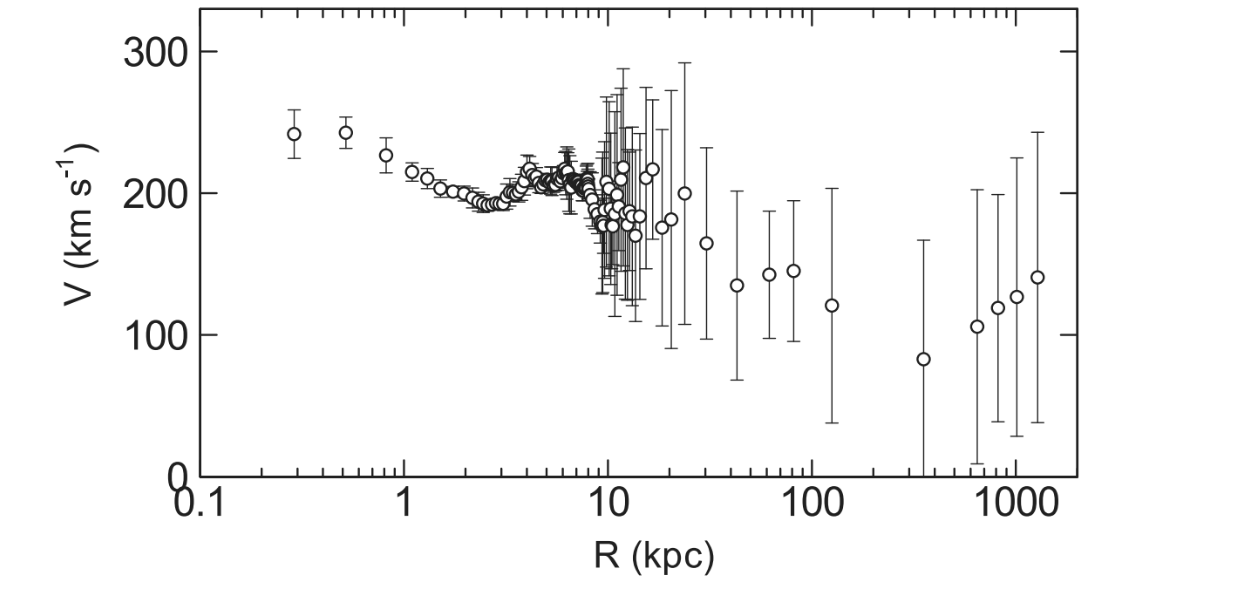
\includegraphics[width=\linewidth]{Sofue_MWtoLGData}
    \caption{Sofue grand rotation curve 2012, }
    \label{fig:mwSofue}
\end{figure}
%Sofue: We included the circular velocities from an SDSS blue stars analysis by Xue et al. (2008; their model 1) by correcting for a systematic difference in the veloc-ities of about 20 km s1, due to our V0 = 200 km s1 instead of their 220 km s1.
%ugggh. have to look at the first two papers to see what assumptions they make. 
%We decomposed the newest rotation curve into a de Vaucouleurs bulge, an exponential disk, and an isothermal dark halo (Sofue et al. 2009).
%OBS METHOD: 
%An inner rotation curve was obtained by a terminal-velocity method applied to radio line observations
% An outer rotation curve was obtained by combining the CO star line velocities and the optical distances
%and by the HI disk-thickness method
%de Vaucouleurs bulge of mass Mb = 1.8 1010 Mˇ with a scale radius of Rb = 0.5 kpc, an exponential disk of mass Md = 71010Mˇ with a scale radius of Rd = 3.5 kpc,
%In the inner Galaxy at R .10 kpc, the rotation velocity is predominantly determined by the bulge and disk contributions, and R < 0.5 kpc it is almost determined by the bulge alone.

  In  recent large surveys of millions of  stars in the Milky Way disk,  we begin to see  constraints to these models from  SDSS APOGEE-2 \citet{2022ApJS..259...35A}, \citet{2010ApJ...716....1B}.
  
  We test our RCFM against three MW models;  a hybrid model from \cite{Xue}, \cite{Sofue}, a model from Stacy McGaugh, and one from (?) Mario Juric, as summarized in Table ~\ref{tab:my_label}.
   \begin{table*}[h!]
      \centering
      \begin{tabular}{|c|c|c|}
        Author & Position of the Solar system   &  scalelength disk\\
        \hline
        Sofue \cite{Sof11}   & 8 kpc &\\
             \hline
        McGaugh\cite{2021DDA....5240103M} & &
      \end{tabular}
      \caption{Citations}
      \label{tab:my_label}
  \end{table*}
  
  {\color{teal} \rule{\linewidth}{0.5mm}}
{\color{teal} \rule{\linewidth}{0.5mm}}
NOTES:  Ask Mario,  Rene y Stacy  \\

  RC for the MW with his mass models. 
 Anatoly - do we still have this data?
  \begin{figure}
    \centering
    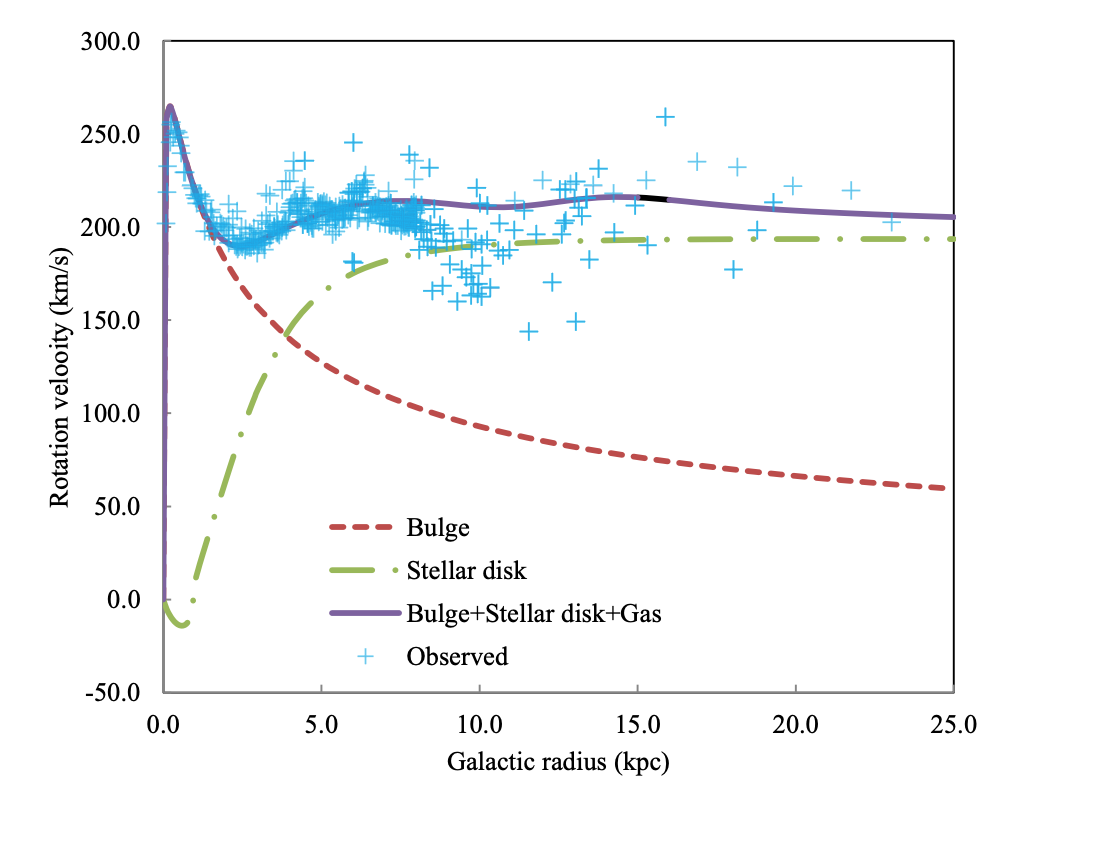
\includegraphics{MW_Enbang_Li}
    \caption{Enbang Li \cite{Li2016ModellingMD}}
    \label{fig:my_label}
\end{figure}

{\color{teal} \rule{\linewidth}{0.5mm}}

 {\color{red} \rule{\linewidth}{0.5mm}}
  %\cite{2010ApJ...716....1B}The Seventeenth Data Release of the Sloan Digital Sky Surveys: Complete Release of MaNGA, MaStar, and APOGEE-2 Data}
  
   %Mario paper \cite{2010ApJ...716....1B} MW tomography to kinematics, but no rotation curve. ask him.
   
  % old Binney article 2012  \cite{10.1093/mnras/stt814}. 
 %ANALYSIS
 \subsubsection{SOFUE XUE MW}
 Sofue MW paper I: \cite{sofue2009unified}, 
 Sofue MW paper II: \cite{10.1093/pasj/61.2.153}
 have params for the Sofue Paper III. (where our MW Scatter data comes from. 
 Xue is a subset of same data, from Sofue Paper III \cite{Sof11}.
 %''A grand rotation curve of the Milky Way Galaxy was constructed, which covers a wide range of radius from the Galactic Center to  1 Mpc, and was deconvolved into bulge, disk, and halo components by least-squares fittings. 
%We determined the masses and scale radii of the bulge and disk to be $Mb = (1.652 ̇ 0.083)  1010Mˇ$, $ab = 0.522  ̇ 0.03$7 kpc,$$ Md = (3.41  ̇ 0.41)  1010$Mˇ, an$d ad = 3.9  ̇ 0.35 kpc. The dark halo was fitted by the Navaro–Frenk–White (NFW) density profile,  = 0=[(R=h)(1 + R=h) 2], and the fit yielded h = 12.5  ̇ 0.9 kpc and0 = (1.06  ̇ 0.14)  102Mˇ pc3. The local dark-matter density near the Sun at R0 = 8 kpc was estimated to be ˇ0 = (6.12  ̇ 0.80)  103 Mˇ pc3 = 0.235  ̇ 0.030 GeV cm3. The total mass inside the gravitational boundary of the Galaxy at R  385 kpc, a half distance to M 31, was estimated to be Mb+d+h = (7.03  ̇ 1.01)  1011 Mˇ. This leads to a stellar baryon fraction of Mb+d=Mb+d+h = 0.072  ̇ 0.018.''
  
 




%ANALYSIS MCGAUGH MW
%ANALYSIS MARIO MW
Mario y company: study of the SDSS stars
\cite{2010ApJ...716....1B}

{\color{teal} \rule{\linewidth}{0.5mm}}


 





\cite{2008ApJ...673..864J} Mario Juric's paper - has info  on the MW from SDSS, surveyed like 48,000 stars. Ask him to look at our MW models. 


 

IN \cite{Li2016ModellingMD} the bulge is more like Sofue. Not flat like McGaugh. 
To understand why. 
``using the recently released Gaia billion-star map8
, we propose a
Galactic disk mass distribution model which is based on the star density distribution
rather than the brightness and mass-to-light ratio. ''
TROUBLE: ``we obtain a flat rotation curve
which reproduces the key observed features with no need for a dark halo''.


 
\subsection{Geometry and Mass-to-light ratios}
 
  Stellar bulges are assumed to be spherical, and stellar disks are assumed to go to exponentially approach zero at  infinity unless there is a clear delineation of the end of the galaxy disk. It is interesting to note that \citet{2016Lelli} state that errors come from uncertainties in the M/L ratios rather than the geometry assumptions
   
   
 
 van Albada: Assume a galaxy is composed of a stellar bulge and a disk, and assume that each has a constant M/L ratio. At 1/3 the effective radius (half light radius) the maxima of the rotation curve happens for spheroid and disk. 
   with  the RCFM in order to compare results with    MOND and RAR and dark matter fits to the same data set   \cite{McGaugh_2014,Li_2018}. 

  In addition, dark matter is not required in the inner rotation curve, where stellar mass is sufficient to explain rotations. 
 
 
   
Photometry 
 is a measure of   a  galaxy's luminosity, which   after processing   through a Population Synthesis Model \cite{BelldYong,10.1093/mnras/sty3223}, gives an estimate of the  baryonic mass components of the galaxy. These mass components, stellar bulge and disk and gas halo, then     yield   Keplerian velocities 
   from Poisson's equation, which fall-off outside of the stellar contributions. 
   
   
 All terms in $\Phi(r)$ used in this paper  are    integrated from estimates of the baryonic mass, as reported in the      SPARC  library \cite{2016Lelli}.  
   Assumptions in their reported luminous mass models  are included in Sec.~\ref{sec:analysis}
Studies of the mass-to-light ratios in galaxies began with Schwarzschild's early investigations \cite{1954AJ.....59..273S} and have evolved into a set of best practices, but modeling of the 
dark matter halo remains severely   under-constrained with correlated parameters including radius, slope, scale length, and halo core radius.     
The technique presented here, whether fundamental or no,  has the advantage of replacing the dark matter term  with a product of terms based only on estimates of the luminous mass and   one free parameter.


It is commonly assumed that   the stellar bulge, gas halo and   dark matter halo are spherically symmetric, but that the stellar disk is axially symmetric. We use 
the Schwarzschild metric   for clarity of the construction;  a static, stationary, spherically symmetric solution of Einstein's equations.
Flattened disks produce gravitational potentials which are weaker than a sphere of the same mass\cite{Chatterjee}. However, numerical integration of the disk is a computationally intensive and requires assumptions of  boundary conditions,   relevant physical scales,  etc. which add extra free-parameters\cite{2011A&A...531A..36H}. We 
  introduce the error of spherical symmetry   for the disk to maintain a clear presentation in the plane of the galactic disk, acknowledging  that inside of $r< R/3$, we   overestimate the gravitational potential, and  mass-to-light ratio by approximately $15\%$ (see Fig.~\ref{fig:my_geom}),  where R is the radius of the stellar disk configuration.  (CHECK WITH STACY). 


This introduced error does not change  the line shape, and   does not introduce any artifacts outside of $R/3$, where rotation curves become flat,  as the potentials for disk and sphere are commensurate there. The assumption of spherical symmetry is commonly used   in evaluation of the   rotation curve velocities from integrated potentials \cite{2022A&A...664A..40M,PhysRevD.70.083509}. 
 
\begin{figure}
    \centering
     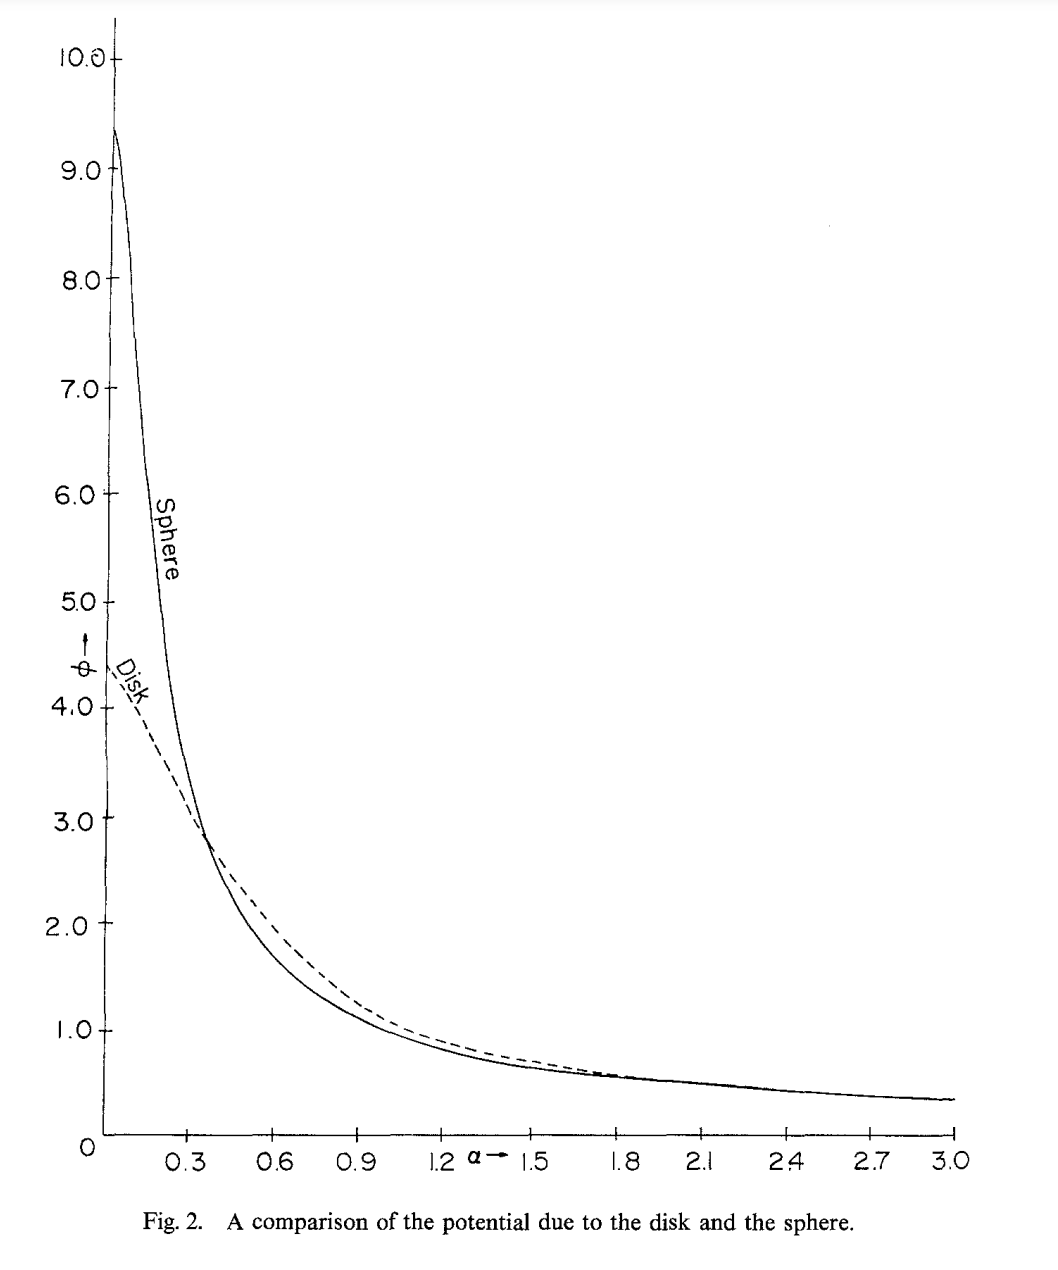
\includegraphics[width=\linewidth]{Chatterjee_SphereDisk.png}
    \caption{ $\alpha = r/R$, for $R$ the radial extent of the stars \cite{Chatterjee}}
    \label{fig:my_geom}
\end{figure}

  
  \subsection{Thing}
We will parametrize gravitational frames from estimates of luminous mass reported kinematically as  $v_{lum}$, Eq.~\ref{eq:zonte1}. These velocities  are constructed from photometric observations of surface brightnesses, interpreted   by a Population Synthesis Model (PSM)\cite{10.1093/mnras/sty3223} as     masses. 
PSM rely upon a complex  suite of  assumptions regarding galaxy evolution, metallicities and initial mass functions  \cite{BelldYong,10.1093/mnras/sty3223}. PSM predict   mass-to-light ratios  $\gamma_i$
 which translate  luminosity into mass as in Eq.~\ref{eq:zonte3}. 
Gas fractions are  not scaled because the observation techniques do not require a PSM to yield masses.  Baryonic mass contributions (disk, bulge and gas) are summed quadratically to represent a mass sum in the same way as in   Eq.~\ref{eq:zonte1}.


  
 
%%%%%%
%%%%%%
%%%%%%%
\section{Analysis and Constraining the free parameter \label{sec:analysis}}
{\color{blue} \rule{\linewidth}{0.5mm}}
 {\color{blue} NOTE TO Rich & Meagan & Amy: Show Stacy  }
{\color{blue} \rule{\linewidth}{0.5mm}}

  
%%TO DO: PUT ASSUMPTIONS FOR SPARC LUM MODELS - " Assumptions in their reported luminous mass models  are included in Sec.~\ref{sec:analysis}. "

In RCFM fits reported here, the    bulge and disk mass-to-light ratios are allowed to vary freely (See Eq.~\ref{eq:zonte3}), though the average values are within stated criteria   \cite{2016Lelli} of $\pm 20\%$. The gas fractions (HI scaled for Helium abundance) are fixed though addition of molecular gas could increase mass fractions in the inner kiloparsec of a galaxy(CITE RENE WB), and it is common (CHECK-Y-YO) to scale the observed 21-cm flux by $4/3$ to account for molecular gas \cite{2004ApJ...609..652M}.


\subsection{NGC 3198 and other galaxies}
\cite{1985ApJAlbada} studies this galaxy, which MOND has troubles with. This galaxy has an exponential disk, they use 2 components -  a thin exponential disk de Vaucouleurs 1959;
Freeman 1970, and dark matter spheroid Young (1976). Dijo algo about using an infinite disk - uggg. 
 
\cite{Toky} mentions that MOND fails to fit NGC 3109, which we fit exceedingly well ($\chi^2 = 0.32$).
%%%%%%
%%%%%%%%
%%%%%%
%%%%%%%
%%%%%%
%%%%%%
\subsection{Correlation to  the model's free parameter }


 In \cite{2016Lelli}, it says that they have fifty  galaxies with highly accurate distance: (45) from tip of the red giant branch, (3) from Cepheids, (2) from supernova, with errors in distance on the order of $5\% - 10\%$. We use this subset to investigate   the free parameters for these galaxies with respect to a guess at its physical significance. 
 
 
 %NEED TO SEE IF WANT TO INCLUDE SN GALS TOO... train the model's free parameter we select a subset of galaxies who have Cepheid or Tip of the Red Giant Branch distance measurements. 
 % DO WE WANT TO DO THIS, OR JUST DO THAT SUBSEQUENT?> When the free parameter is fixed to a constant value, we will then run on the entire SPARC data set,
We also exclude galaxies  which have an inclination greater than $85^o$ as impossible to constrain a proper surface brightness profile, and those at inclinations less than $35^o$ as being impossible to accurately report line of sight Doppler shifts.   
  By this criteria, we select 46 galaxies (See Table \ref{tab:Tset}. 
  
  
  \begin{table*}[]
      \centering
      \begin{tabular}{|c|c|c|c|c|c|}
      \hline \hline
Galaxy Name & Hubble Type(1)& 	Distance (Mpc)&Mean Error on D (Mpc)& 	Distance Method (2)& 	Inc (deg)\\
    \hline \hline\\
CamB&   	10&    3.36&  	0.26&   2&  65\\
D564-8& 	10& 	8.79& 	0.28& 	2& 	63\\
D631-7& 	10& 	7.72& 	0.18& 	2& 	59\\
DDO154& 	10& 	4.04& 	0.2& 	2& 	64\\
DDO168& 	10& 	4.25& 	0.21& 	2& 	63\\
ESO444-G084& 10& 	4.83& 	0.48& 	2& 	32\\
IC2574& 	9& 	3.91& 	0.2&    	2& 	75\\
NGC0024& 	5& 	7.3& 	0.36&   	2& 	64\\
NGC0055& 	9& 	2.11& 	0.11&   	2& 	77\\
NGC0247& 	7& 	3.7& 	0.19&   	2& 	74\\
NGC0300& 	7& 	2.08& 	0.1&    	2& 	42\\
NGC0891& 	3& 	9.91& 	0.5&    	2& 	90\\
NGC1705& 	11& 	5.73& 	0.29& 	2& 	80\\
NGC2366& 	10& 	3.27& 	0.16& 	2& 	68\\
NGC2403& 	6& 	3.16& 	0.16&   	2& 	63\\
NGC2683& 	3& 	9.81& 	0.49&   	2& 	80\\
NGC2841& 	3& 	14.1& 	1.4&    	3& 	76\\
NGC2915& 	11& 	4.06& 	0.2& 	2& 	56\\
NGC2976**& 	5& 	3.58& 	0.18&   	2& 	61\\
NGC3109& 	9& 	1.33& 	0.07&   	2& 	70\\
NGC3198& 	5& 	13.8& 	1.4&    	3& 	73\\
NGC3741& 	10& 	3.21& 	0.17& 	2& 	70\\
NGC4068& 	10& 	4.37& 	0.22& 	2& 	44\\
NGC4214& 	10& 	2.87& 	0.14& 	2& 	15\\
NGC5055& 	4& 	9.9& 	0.3&    	2& 	55\\
NGC5907& 	5& 	17.3& 	0.9&    	2& 	88\\
NGC6503& 	6& 	6.26& 	0.31&   	2& 	74\\
NGC6789& 	11& 	3.52& 	0.18& 	2& 	43\\
NGC6946& 	6& 	5.52& 	1.66&   	2& 	38\\
NGC7331& 	3& 	14.7& 	1.5&    	3& 	75\\
NGC7793& 	7& 	3.61& 	0.18&   	2& 	47\\
NGC7814& 	2&  	14.4& 	0.66& 	2& 	90\\
PGC51017**& 	11& 	13.6& 	1.4& 	2& 	66\\
UGC01281& 	8&   	5.27& 	0.24& 	2& 	90\\
UGC04305**& 	10& 	3.45& 	0.17& 	2& 	40\\
UGC04483& 	10& 	3.34& 	0.31& 	2& 	58\\
UGC07151& 	6& 	6.87& 	0.34&   	2& 	90\\
UGC07232& 	10& 	2.83& 	0.17& 	2& 	59\\
UGC07524& 	9& 	4.74& 	0.24& 	    2& 	46\\
UGC07559& 	10& 	4.97& 	0.25& 	2& 	61\\
UGC07577& 	10& 	2.59& 	0.13& 	2& 	63\\
UGC07866& 	10& 	4.57& 	0.23& 	2& 	44\\
UGC08286& 	6& 	6.5& 	0.21&   	2& 	90\\
UGC08490& 	9& 	4.65& 	0.53&   	2& 	50\\
UGC08837& 	10& 	7.21& 	0.36& 	2& 	80\\
UGCA281& 	11& 	5.68& 	0.28& 	2& 	67\\
UGCA442& 	9& 	4.35& 	0.22& 	    2& 	64\\
UGCA444& 	10& 	0.98& 	0.05& 	2& 	78\\
    \hline \hline           
      \end{tabular}
      \caption{Table from  \citet{2016Lelli}. 
      (1) Hubble type:  from (CITE) de
Vaucouleurs et al. (1991), (CITE) Schombert et al. (1992), or (CITE) NED3
of: 0 = S0, 1 = Sa, 2 = Sab,
3 = Sb, 4 = Sbc, 5 = Sc, 6 = Scd, 7 = Sd, 8 = Sdm,
9 = Sm, 10 = Im, 11 = BCD.  (2) Distance method: : 1 = Hubble flow,
2 = tip of the red giant branch, 3 = Cepheids, 4 = Ursa Major
cluster of galaxies, 5 = supernovae. ** notes galaxies excluded from fit bc fail to fit, and see if we want to include SN gals, there's only 3...and 2 of the 3 that fail are weirdi rotations (non-circular)}
0      \label{tab:Tset}
  \end{table*}
  
  %%NOTE: Homies for SPARC used hybrid rotation curves on 56 galaxies, combining H-alpha  (inner) with HI (outer) Check if our "bad" gals are part of thi, or if is algo mas. Despite the high spatial resolution, Hα rotation curves are sometimes quite uncertain due to the patchy distribution and complex kinematics of Hα gas, especially for low-mass and LSB galaxies. We %use only H I data for the several objects:DDO 154, IC 2574, NGC 3109, NGC 5033, NGC 5055,NGC 6946, NGC 7331, and UGC 2259.(THESE ARE ALL GOOD
  %H I and Hα rotation
%curves, however, agree within the errors

%or face-on ones.We assign a quality flag (Q) to each rotation curve using the following scheme: Q = 1 for galaxies with high-quality H I data or hybrid Hα/H I rotation curves (99 objects); Q = 2 for
%galaxies with minor asymmetries and/or H I data of lower
%quality (64 objects); Q = 3 for galaxies with major asymmetries, strong noncircular motions, and/or offsets between H I
%nd stellar distributions (12 objects). Galaxies with Q = 3 are%
%not suited for detailed dynamical studies: we build mass models
%for completeness but do not consider them in our analysis.
%K BIEN_ Both UGC04305_rotmod and PGC51017_rotmod have Q=3. discard anyhow. but not: NGC2976_rotmod, it's a Q=2. Plus we have a few other galaxies in this subset with a Q=3,,,


  We search the free parameter $\alpha$ space of this subset of SPARC galaxies by plotting the single valued free parameter of each galaxy   versus a proxy for the gradient in the gravitational potential
  
   \begin{equation}
     \rho = L_{total}/R_{eff}.
 \end{equation}
 
 The  estimates of the  total luminosities $L_{total}$ at $3.6 \mu m$,  assume a solar
absolute magnitude of 3.24 at $3.6 \mu m$ (CITE Oh et al. 2008). The effective radius $R_{eff}$ is    the radius encompassing half of the total luminosity \citet{2016Lelli}.  
 

 We find $\alpha$  to be   strongly correlated to  this quantity. 
  
 \begin{figure*}[h]
\scalebox{0.5}%
{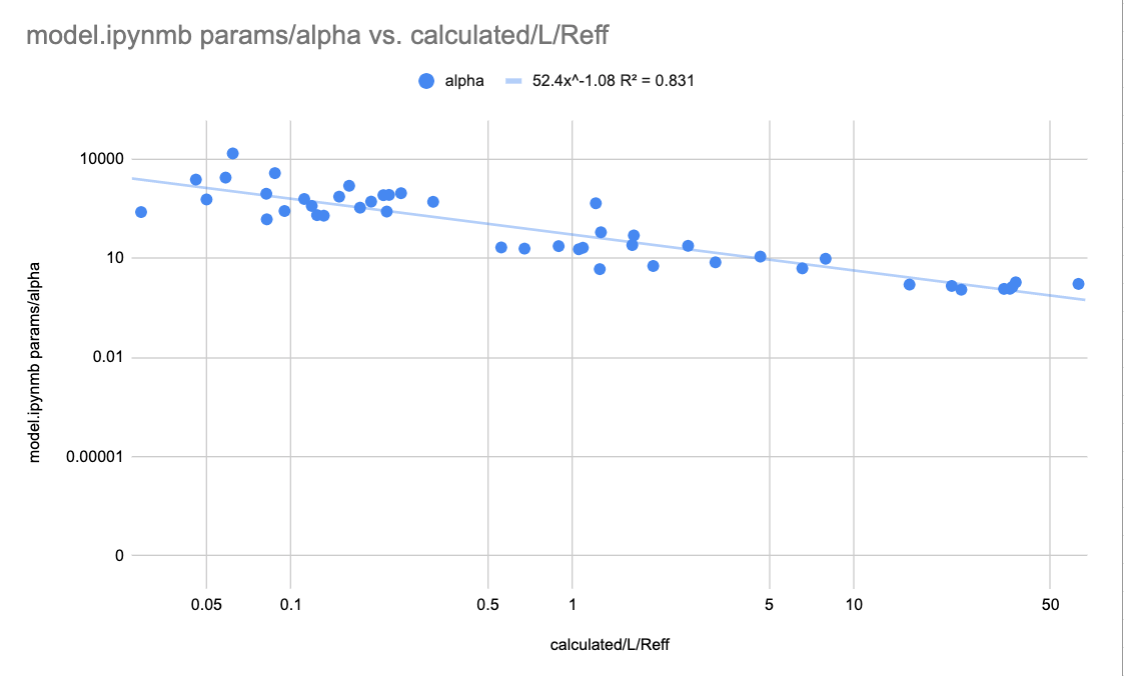
\includegraphics{alpha_10_18_22.png} }
\caption{ Remake this graph, nice   }
\label{alpha2}
\end{figure*}  
 
for 
\begin{equation}
    \alpha = 
\end{equation}



We might assume that $\alpha$ is a ratio of the same quantity for  the Milky Way $\rho_{mw}$ with respect to the other   galaxy $\rho_{gal}$  

\begin{equation}
\alpha=\left(\frac{\rho_{mw}}{\rho_{gal}}\right)^{b}  ,
\label{correl}
\end{equation}

then we arrive at a similar fit (See Fig.~\ref{alpha1}.

 
\subsection{MOND  \& RAR Comparison}



 
 In MOND,  classical gravity is transitioned to  a paradigm where the luminous mass is the only mass  but    the acceleration scale of gravity changes on the enormous distance scales of galaxies. MOND amounts to a phenomenological law of galaxy rotation curves, though does struggle in some galaxies.  Relativistic extensions of MOND have been summarized by  \citet{Famaey2012} and include notably the work of CITE(BEKENSTEIN), though all approaches require modifications to Einstein's well tested gravitational theory (CITE). 
  BY transitioning the MONDian concept of changing acceleration scales to changing  relative curvatures, we implicitly replace MOND's acceleration scale with the baryonic potential of the Milky Way, and find a more 
  efficient and flexible model than MOND. We are successful at fitting galaxies at Cepheid distances (GIVE NAME) that MOND struggles with, and we propose that this increased power is due to the more flexible use of the changing acceleration scale when pinned to the Milky Way and allowed to be the other frame in all transformations. 
  
While reported error    estimates on rotation curve velocities  have not been standardized across the field~\citep{Blok,Gent},     one can reliably   compare fits to the same data with the same  errors. The     reduced $\chi^2_r$ values printed on each graph and in table (MAKE TABLE), demonstrate the higher efficacy of the RCFM. 
 
  \citet{McGaugh2016RAR} is the paper where they present new fitting formula (compare to MOND), but en verdad, no me importa a mi. 
  
 
 
 
 
% \cite{McGaugh2016RAR} is the other one. This one describes the sample. 175 SPARC galaxies. Describes all the assumptions for the disk, gas, bulge models, the band used and reasoning, rotation curve data from HI, 
 
% They only fit a subset (153 of 175) of these galaxies.I get 128, I guess I'm cutting endpoints of 85 and 30 and they include. Plus I exclude like five that I think fail to fit
 
 
 \section{  Conclusions \label{sec:conclu}  }
 

{\color{red} This heuristic replacement of dark matter is not a fundamental derivation, but    one supposes if it is possible to quantify these
excesses in shifted spectra using only luminous mass as we do in this paper,  then a       derivation from first principles should   exist.  The curious conspiracy of the luminous mass to   determine the dark matter  is here more compactly explained and characterized as the imprint of our Milky Way on Doppler shifted spectra we receive from external galaxies. Not only is this a more efficient way to predict rotations curves as judged by the average reduced $\chi^2$, but it is also a  more conservative choice than either MOND or dark matter which both require new physics \cite{de_Blok_2010}.  
  
 
 

  
 
%Places where dark matter is invoked. Structure formation: put spherical model replace flat, solve. Galaxy clusters, same,put flow lines on surfaces supported by dark energy. Tully Fisher: temp dependence with mass - but read Beckenstein's description carefully. Hemakes some points.  
   
 
We   present here a new picture of flat-rotation curves which does not   modify Einstein gravitational physics, but adds a new technique to the standard transformations of   relativity. }
  
 

%%%%%%
%%%%%
%%%
%%
%
%%%%%%


 % \caption{Results   for SPARC Luminous mass profiles  [NOT UPDATED]\label{sumRESULTS}}
 % \begin{tabular}{@{}llccccccc@{}}
 % \hline
 %  Galaxy     	  &Ref.~&  \multicolumn{3}{c}{\underline{ Other Model Fit Results}}	& & \multicolumn{3}{c}{\underline{LCM Fit Results }}  \\
%\hline
%   	 	& & &  $M/L_{disk}$		& $\chi^2_r$	&&$M/L$&$r_e$&$\chi^2_r$ \\ 
% \hline
%F 563-1	& 2	%& 			
%					&NFW	&--	 		&-- & 	&1.13 	&2.84 	&0.06 \\
%M 31* 	& 12 	%&7.5
%					&ISO	 	 &7.50		&0.36 & 	&5.88	 &4.80 	&0.04  \\
%M 33		& 5	 %&	K 		
%					& NFW 	&0.70		&2.46&  	 &1.98	 &1.46	& 0.17 \\
%NGC 891*	& 11 	% &3.6$\,\umu$m 
		%			&MaxLight &0.9 			&1.10  & 	 &--  	 &	&0.25 \\ 
%NGC 925 	&3	%&3.6$\,\umu$m
 			%		&ISO 	&0.18		 &2.40& 	&0.92	 &4.35	&0.11 \\
%NGC 2403	 & 3	%& 3.6$\,\umu$m
		%			& NFW	&0.41 	 	&4.56& 	&1.12	 	&2.18		& 0.88 \\
%NGC 2841*  &6-3	% & 3.6$\,\umu$m
%					&  James	&0.74 	 	&0.45 & 	&6.25	  &4.84	&0.11 \\
%NGC 2903  &10	 %&B	   		
%					&MOND   	&3.60 	 	&10.71& 	 &2.2	 	&2.81		&0.47\\
% NGC 3198 & 3 	%&3.6$\,\umu$m
%					 &NFW	&0.80	   	&5.40  &   	 &1.80 	 &5.10	&0.64   \\
%NGC 3521  & 8-6	 %&3.6$\,\umu$m 
%					&MOND	&0.71 	 	&0.97 & 	 &2.13  &3.23	&0.22 \\
%NGC 3726	& 10	%&B 			
%					&MOND	&1.00	 	&3.57& 	&1.06	 &2.70	&0.05 \\
%NGC 3953	& 10	%&B 			
%					&MOND	&2.7		 	&1.35& 	&1.79 	&2.60 	&0.35 \\
%NGC 3992	& 10	%&B 			
%					&MOND	&4.93	 	&0.50& 	&2.45 	 &4.77	&0.04 \\
%NGC 4088	& 10	%&B 			
%					&MOND	&1.16		 	&1.70& 	&5.58	 &2.70	&0.27 \\
%NGC 4138	& 10	%&B 			
%					&MOND	&3.5		 	&2.12& 	&3.67	 &1.46	&0.01 \\
%NGC 5055*	 & 3	%&3.6$\,\umu$m 
%					&  NFW	&0.79	 	&17.23&  	&5.87	 &3.29	&0.69 \\
%NGC 5533*	 & 10 %&B 			
%					&MOND	&0.6		  	&1.57 & 	&7.11 	  &3.23	&0.22  \\
%NGC 5907*	& 10	%&B 			
				%	&MOND	&1.6 		 	 &0.44& 	&2.04	 &3.45	%&0.09 \\
%NGC 6946*	&  10	 %& B			
%					&  MOND	& 0.5		 	&   3.03& 	&1.44 	 &0.76	&0.07  \\ 
%NGC 6946*	&  3	 %& B			
%					&  NFW	& 0.5		 	&   3.03& 	&1.44 	 &0.76	&0.07  \\ 
%NGC 7331	&8	% & 3.6$\,\umu$m
%					&James	&0.4 		 	& 0.45& 	&1.34	 &2.44	&0.09 \\
%NGC 7793  &14	%&B			
%					&ISO		&2.6		 	&1.08& 	&2.7	 &1.51	&0.11 \\
%NGC 7814* &11 	% & 3.6$\,\umu$m
%					&ISO   	& 0.68  	 	& 0.25& 	 &-- 	   &	&0.20 \\ 
%UGC 128		&6	%&				
	%				&James	&			&	&	&1.58	  &10.3	%&0.20\\
%UGC 6973	& 10	%&B 			
%					&MOND	&2.7		 	&23.5 & 	&--  	& 	&0.06 \\
%UGC 7524	& 6	%&B 			
%					&James	&--		 	&-- & 	&2.10 	&3.32 	&0.06 \\
% 1.~\citet{Bege}, 2.~\citet{JNav}, 3.~\citet{Blok} , 4.~\citet{Maria}, 
%5.~\citet{Cor03}, 6.~\citet{James},   7.~\citet{Batt},   8.~\citet{Gent},   9.~\citet{Bot},   10.~\citet{SanMcGa},
 % 11.~\citet{Frat},   12.~\citet{Car},   13.~\citet{giraud2000universal},   14.~\citet{Dicaire}, %15.~\cite{Klypin}. \\
%    \end{minipage}
%\end{table*} 


   

  \section[]{Acknowledgments}
 This work is dedicated to Emmett Till, and was written on the usual and accustomed lands of the Coast Salish Peoples in Washington State, and those of the Cheyenne, Arapaho and Ute Tribal Peoples in Colorado, with    respect and gratitude.

  The authors would like to thank  S.\ McGaugh,  V.\,P.\,  Nair,   R.\, Walterbos,  A.\, Klypin, K. Bender, C. Beetle and     T.\, Boyer.   \\
  
 
% QUESTION FOR GROUP: how is our model predictive, more so than MOND, since we both do well on fitting galaxies. The Milky Way. We get a large enough sample of galaxies with certain distances and good photometry (SPARC) and run against a two MW. 



 \begin{figure}[h]
\begin{subfigure}{.5\textwidth}
  \centering
  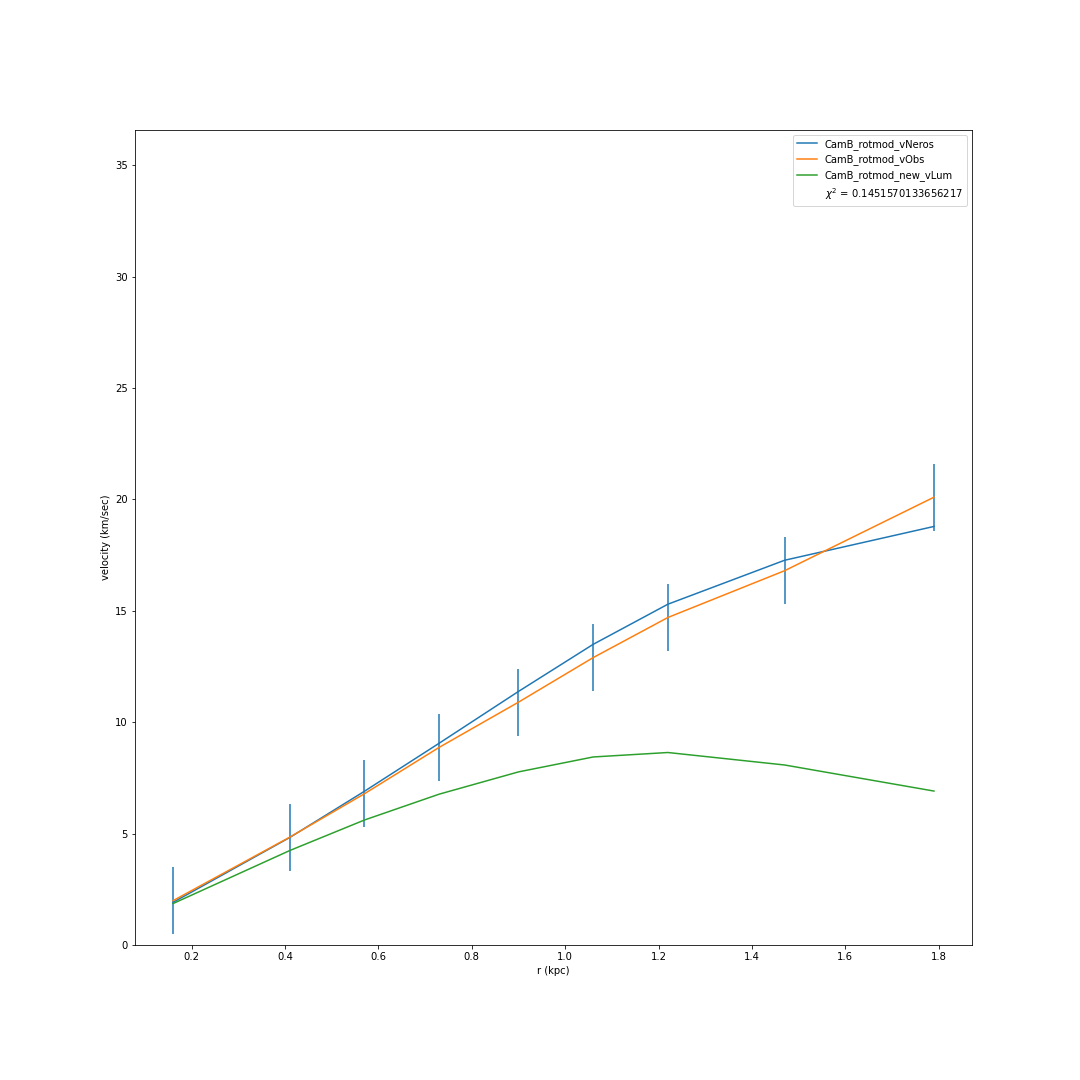
\includegraphics[width=.8\linewidth]{figures/CamB_rotmod_XueSofue.png}
  \caption{SPARC\cite{2016Lelli}}
  \label{fig:sfig1}
\end{subfigure}%
\begin{subfigure}{.5\textwidth}
  \centering
  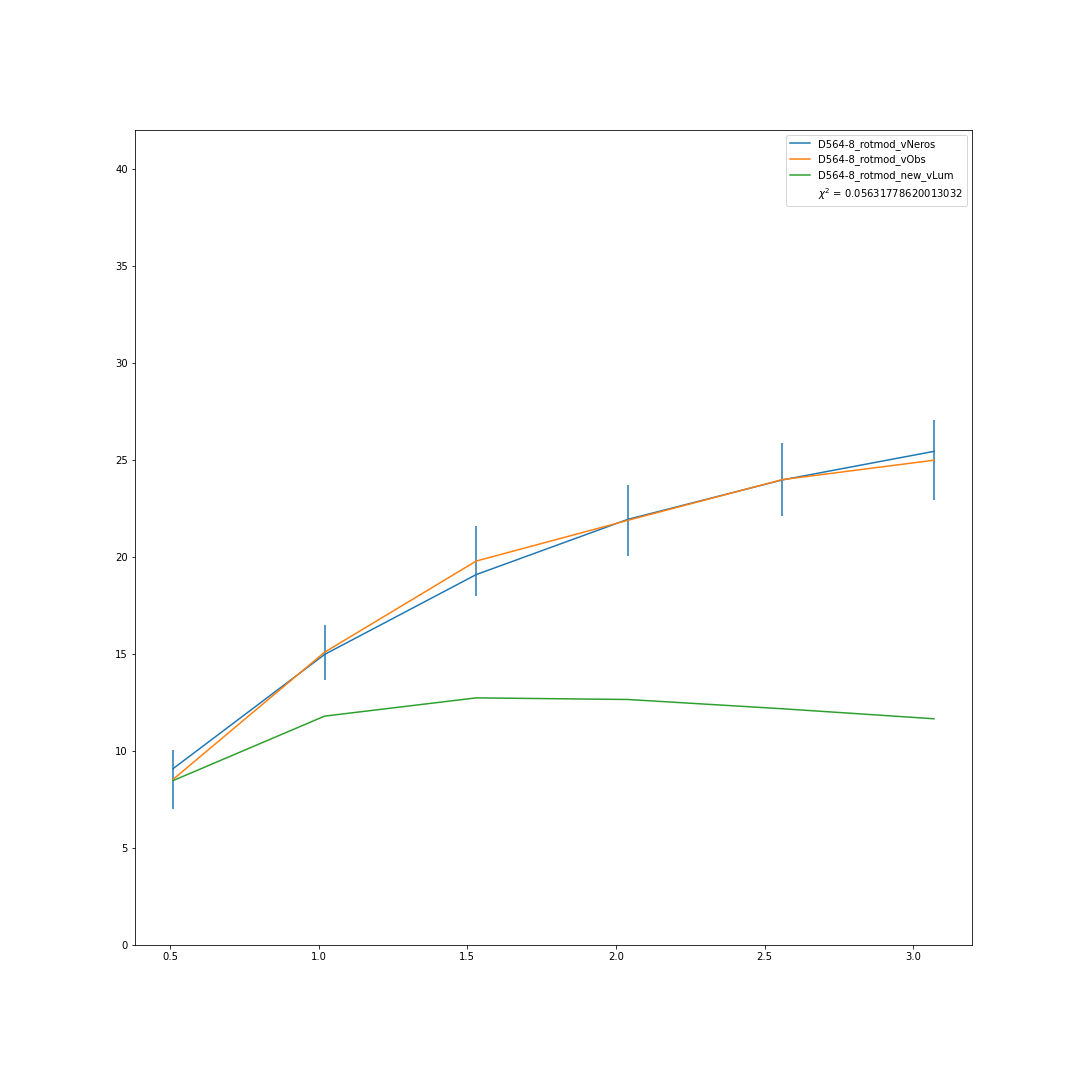
\includegraphics[width=.8\linewidth]{figures/D564-8_rotmod_XueSofue.png}
  \caption{D564-8}
  \label{fig:sfig2}
\end{subfigure}
\begin{subfigure}{.5\textwidth}
  \centering
  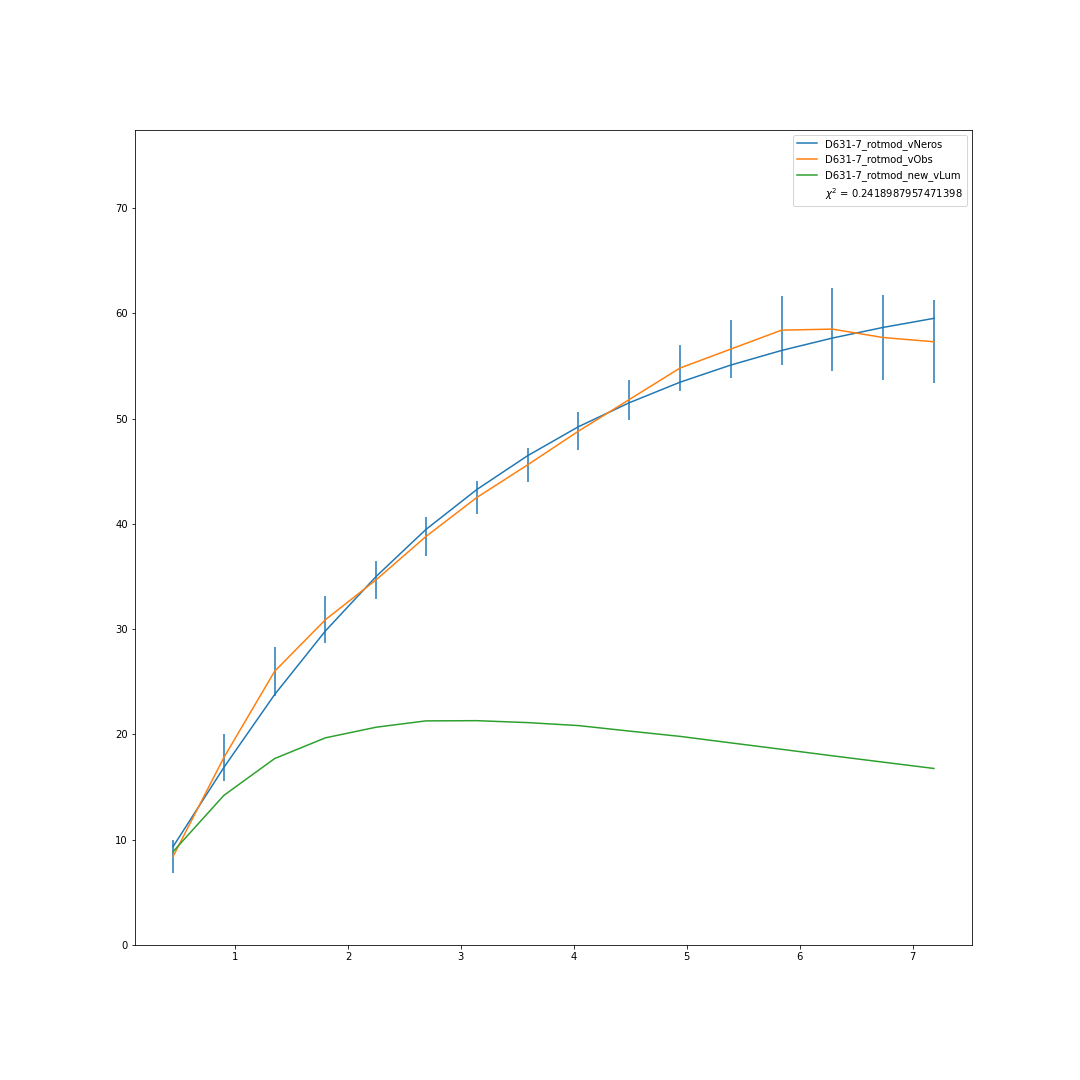
\includegraphics[width=.8\linewidth]{figures/D631-7_rotmod_XueSofue.png}
  \caption{D631-7}
  \label{fig:sfig3}
\end{subfigure}
\begin{subfigure}{.5\textwidth}
  \centering
  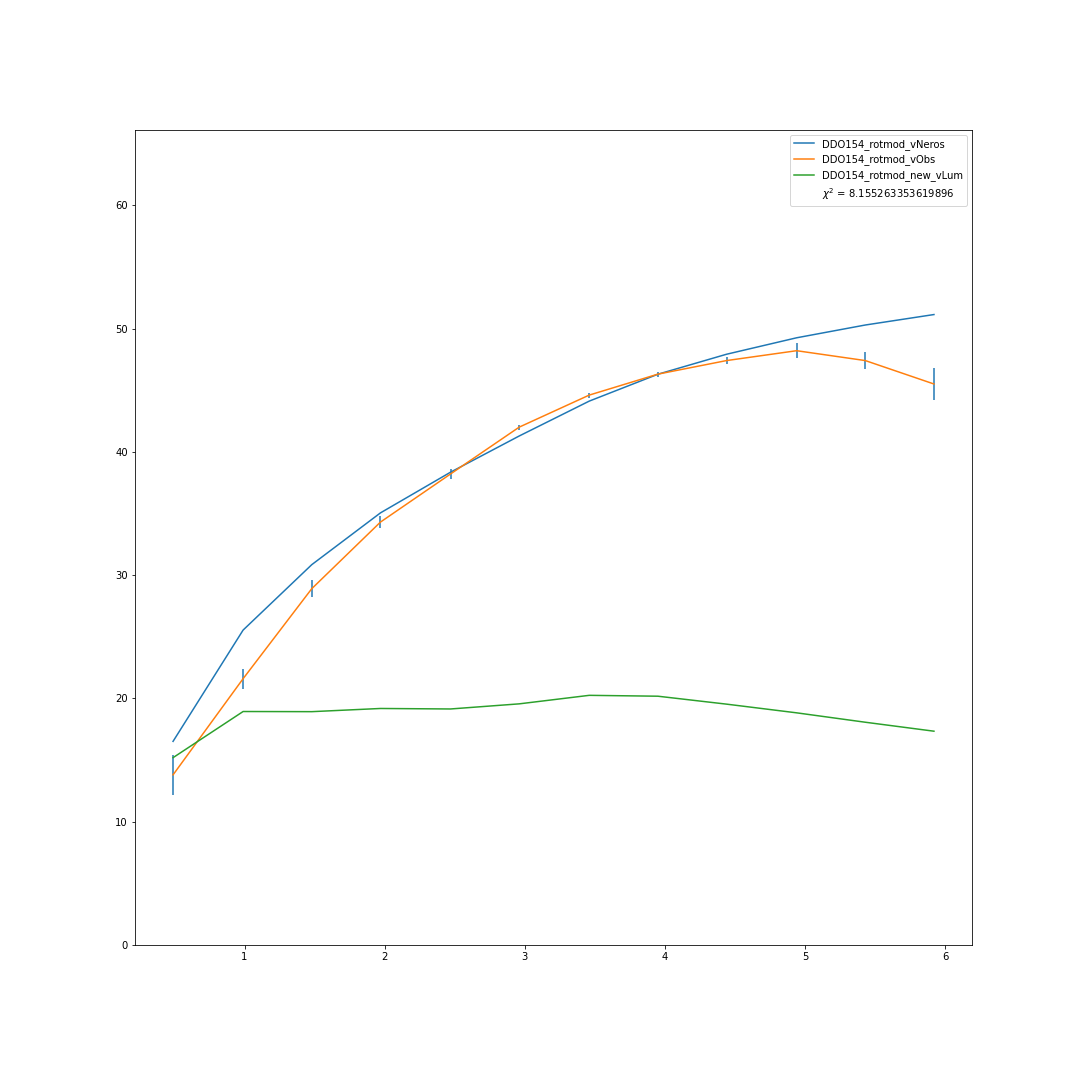
\includegraphics[width=.8\linewidth]{figures/DDO154_rotmod_XueSofue.png}
  \caption{DDO154}
  \label{fig:sfig4}
\end{subfigure}%
\begin{subfigure}{.5\textwidth}
  \centering
  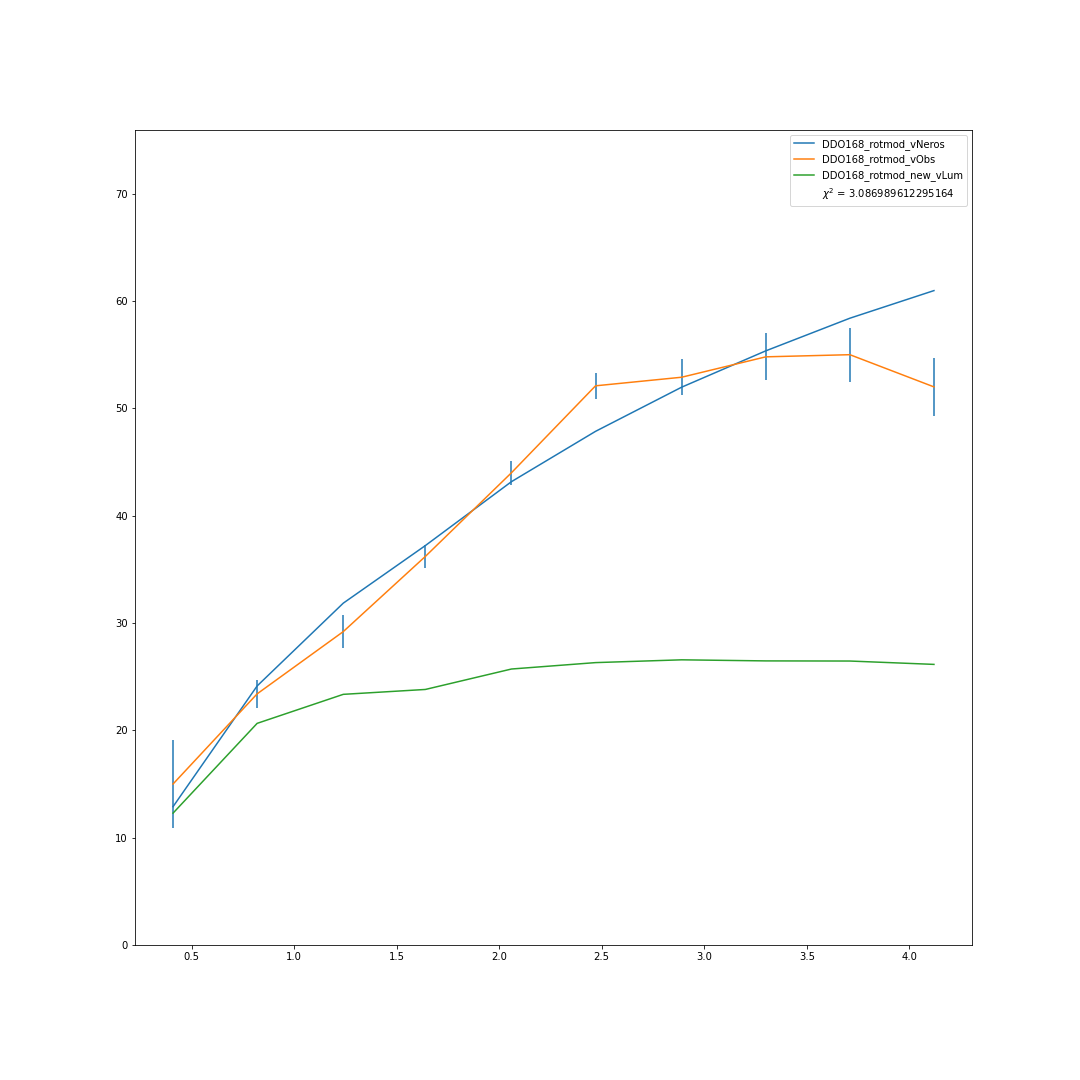
\includegraphics[width=.8\linewidth]{figures/DDO168_rotmod_XueSofue.png}
  \caption{DDO168}
  \label{fig:sfig5}
\end{subfigure}
\begin{subfigure}{.5\textwidth}
  \centering
  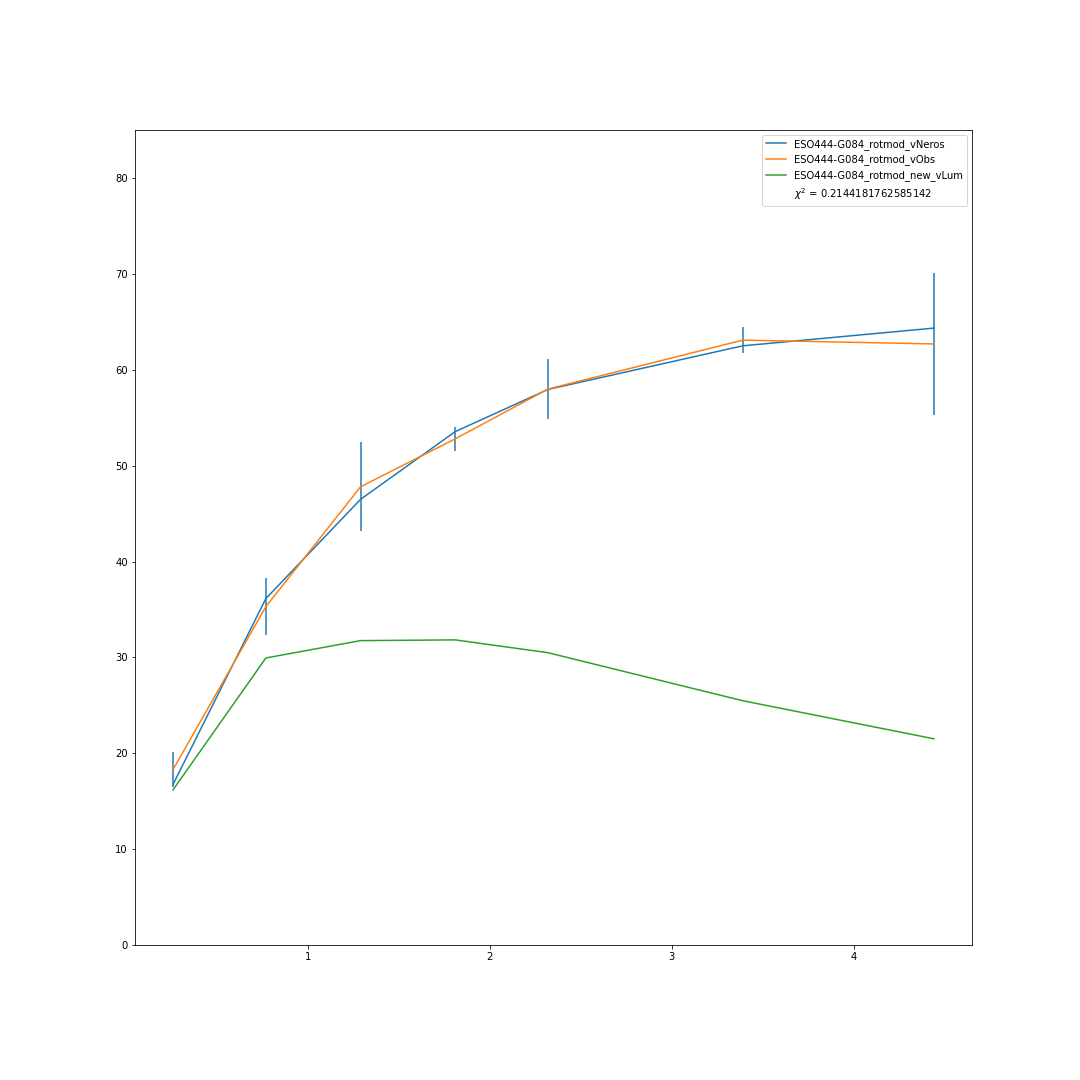
\includegraphics[width=.8\linewidth]{figures/ESO444-G084_rotmod_XueSofue.png}
  \caption{ESO444-G084}
  \label{fig:sfig9}
\end{subfigure}%
\end{figure}

\clearpage
  \begin{figure}[h]
\begin{subfigure}{.5\textwidth}
  \centering
  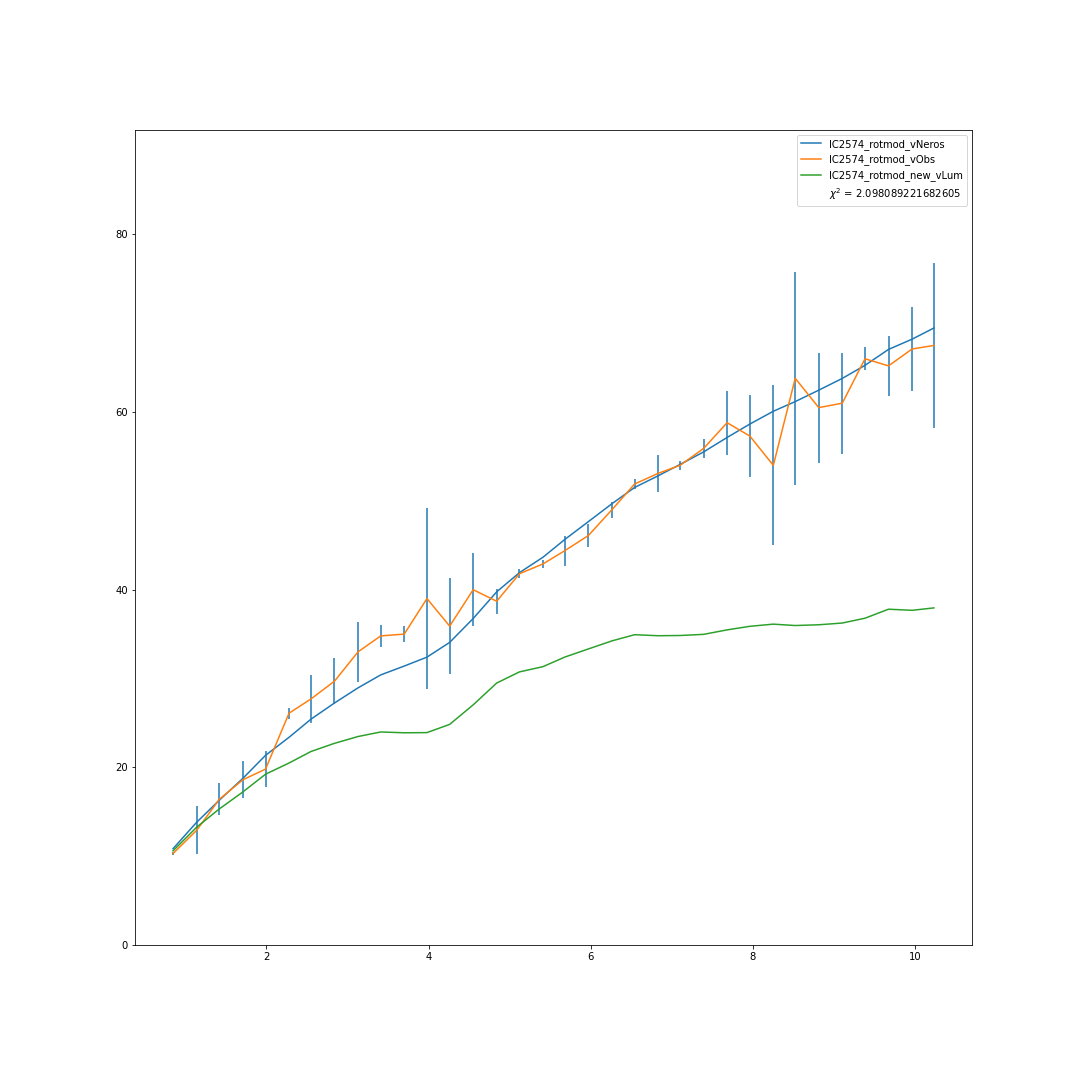
\includegraphics[width=.8\linewidth]{figures/IC2574_rotmod_XueSofue.png}
  \caption{IC2574}
  \label{fig:sfig10}
\end{subfigure}
\begin{subfigure}{.5\textwidth}
  \centering
  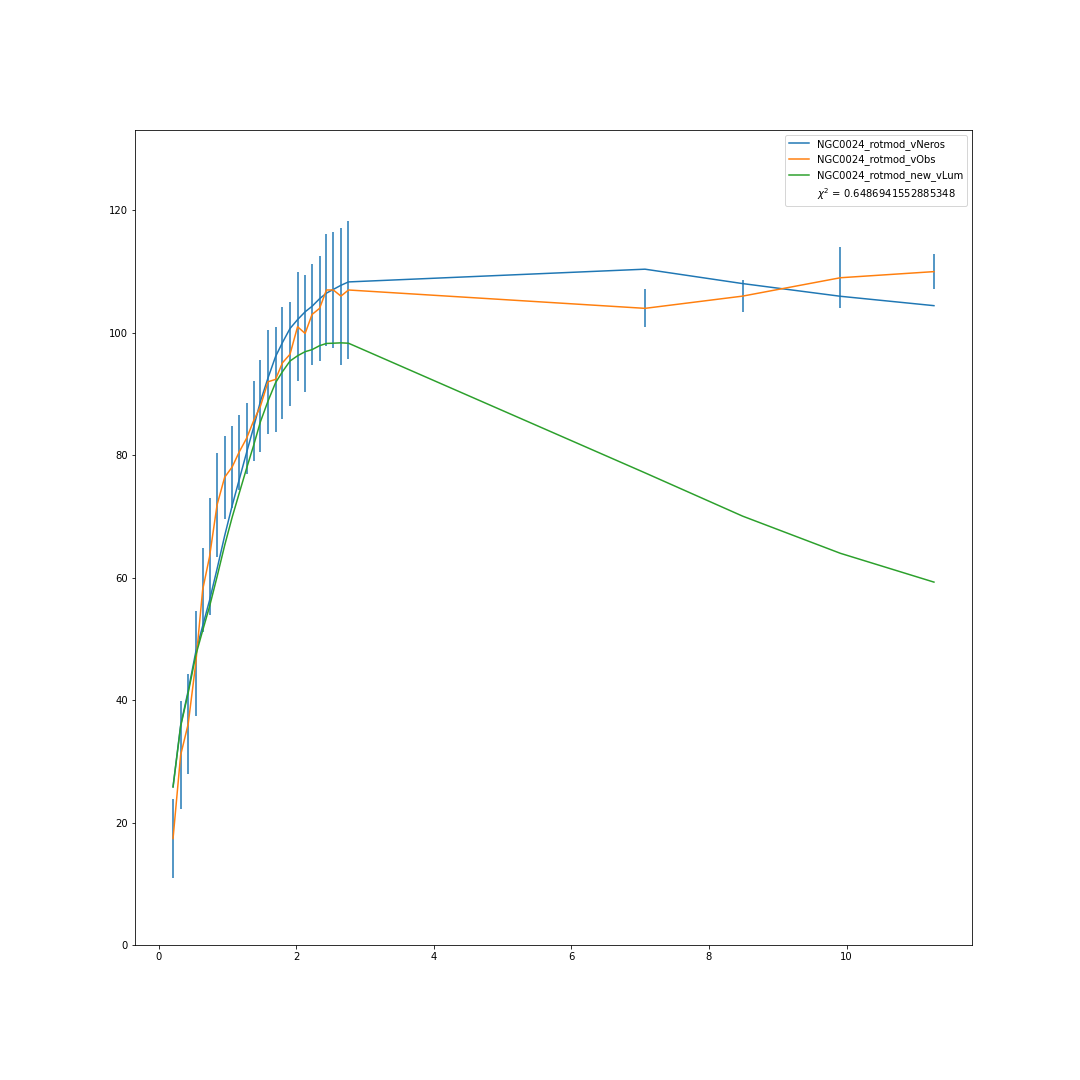
\includegraphics[width=.8\linewidth]{figures/NGC0024_rotmod_XueSofue.png}
  \caption{NGC0024}
  \label{fig:sfig6}
\end{subfigure}%
\begin{subfigure}{.5\textwidth}
  \centering
  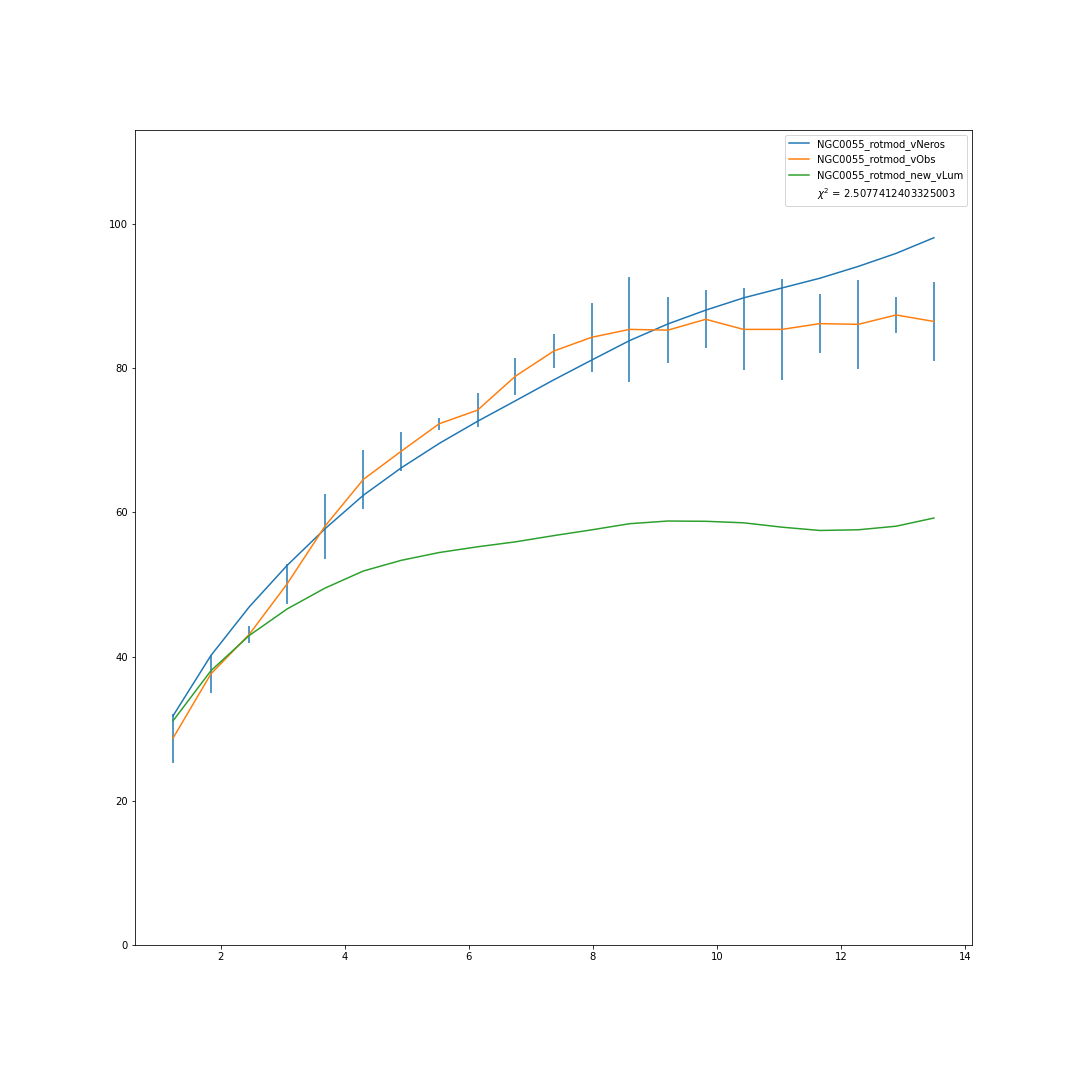
\includegraphics[width=.8\linewidth]{figures/NGC0055_rotmod_XueSofue.png}
  \caption{NGC0055}
  \label{fig:sfig7}
\end{subfigure}
\begin{subfigure}{.5\textwidth}
  \centering
  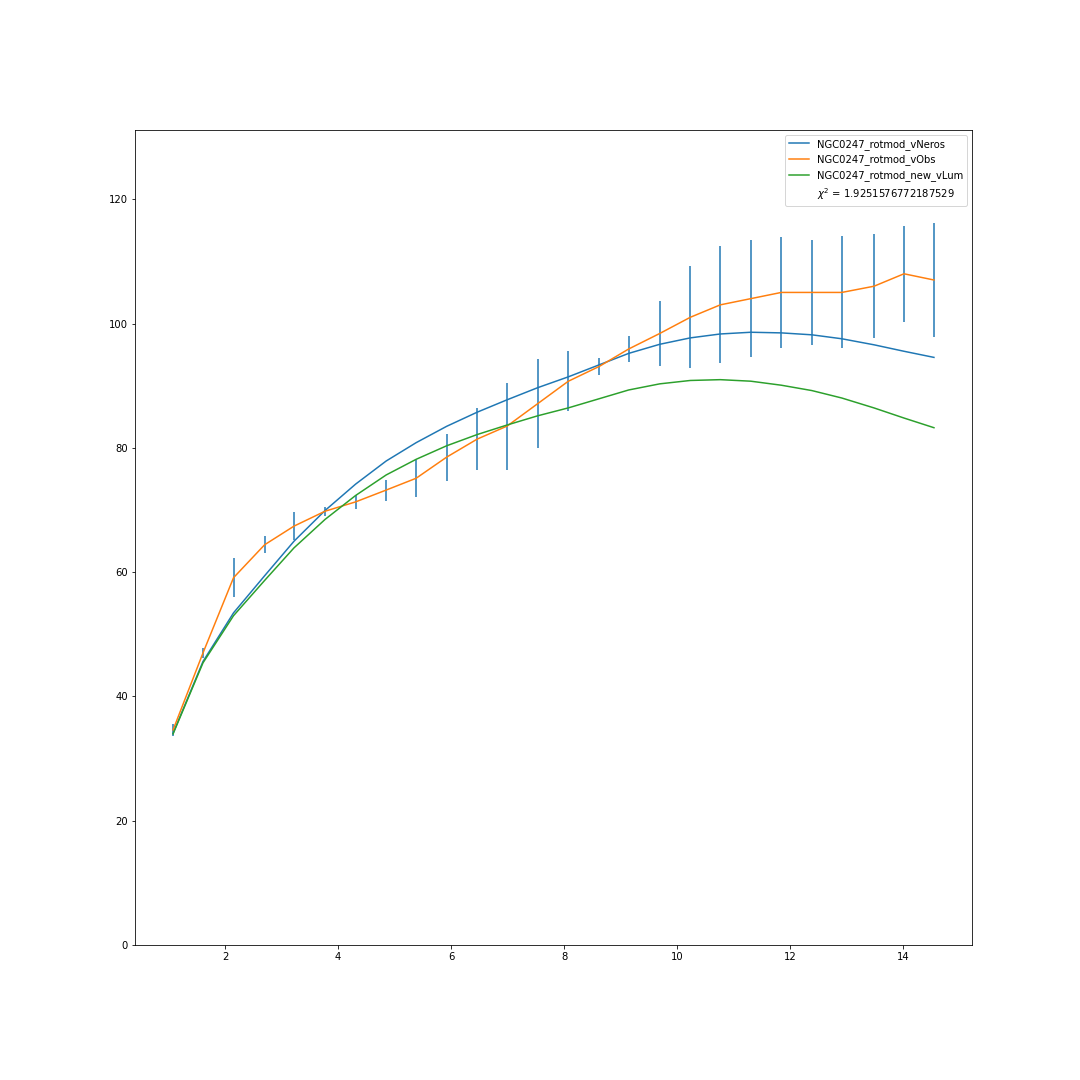
\includegraphics[width=.8\linewidth]{figures/NGC0247_rotmod_XueSofue.png}
  \caption{NGC0247}
  \label{fig:sfig8}
\end{subfigure}
\begin{subfigure}{.5\textwidth}
  \centering
  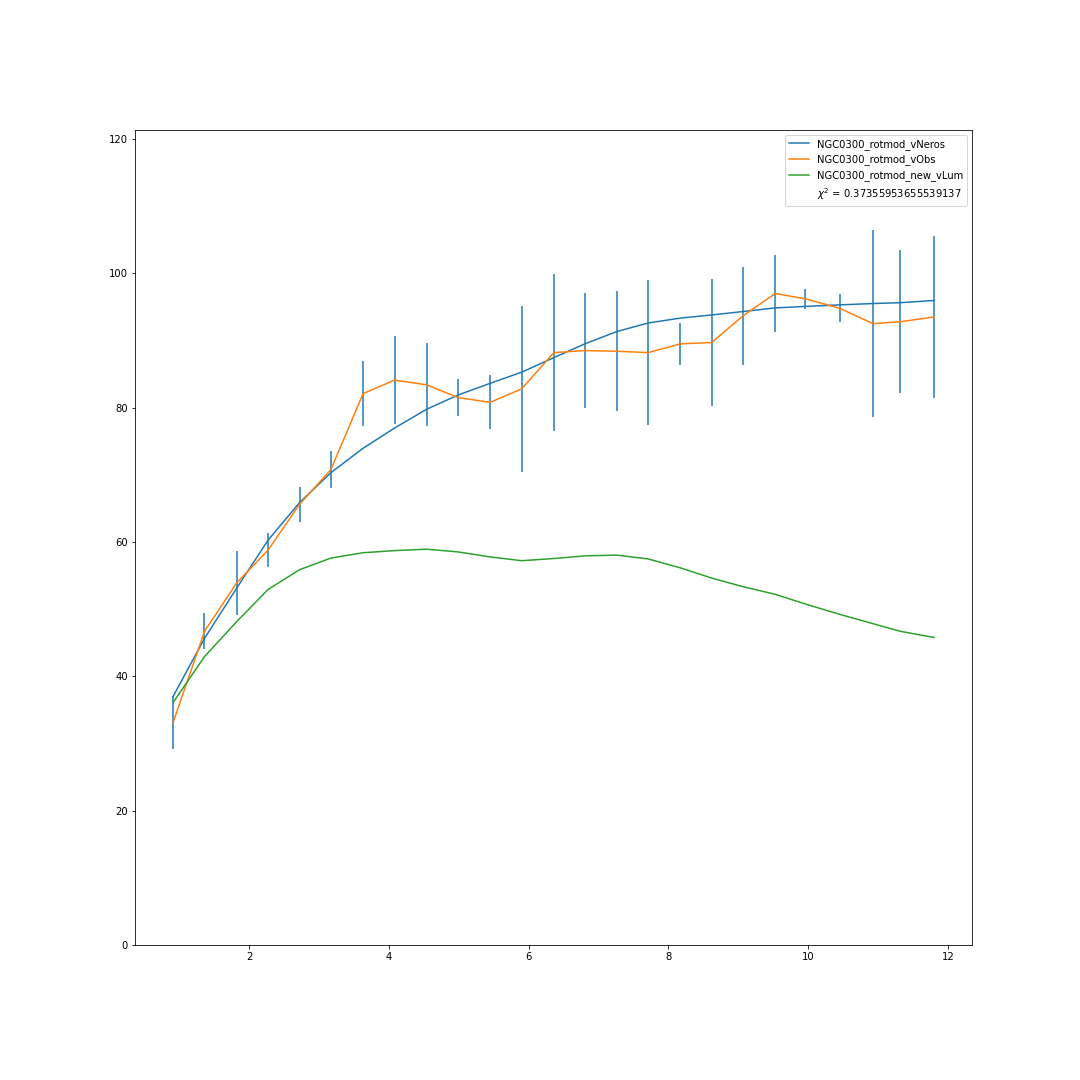
\includegraphics[width=.8\linewidth]{figures/NGC0300_rotmod_XueSofue.png}
  \caption{NGC0300}
  \label{fig:sfig11}
\end{subfigure}%
\begin{subfigure}{.5\textwidth}
  \centering
  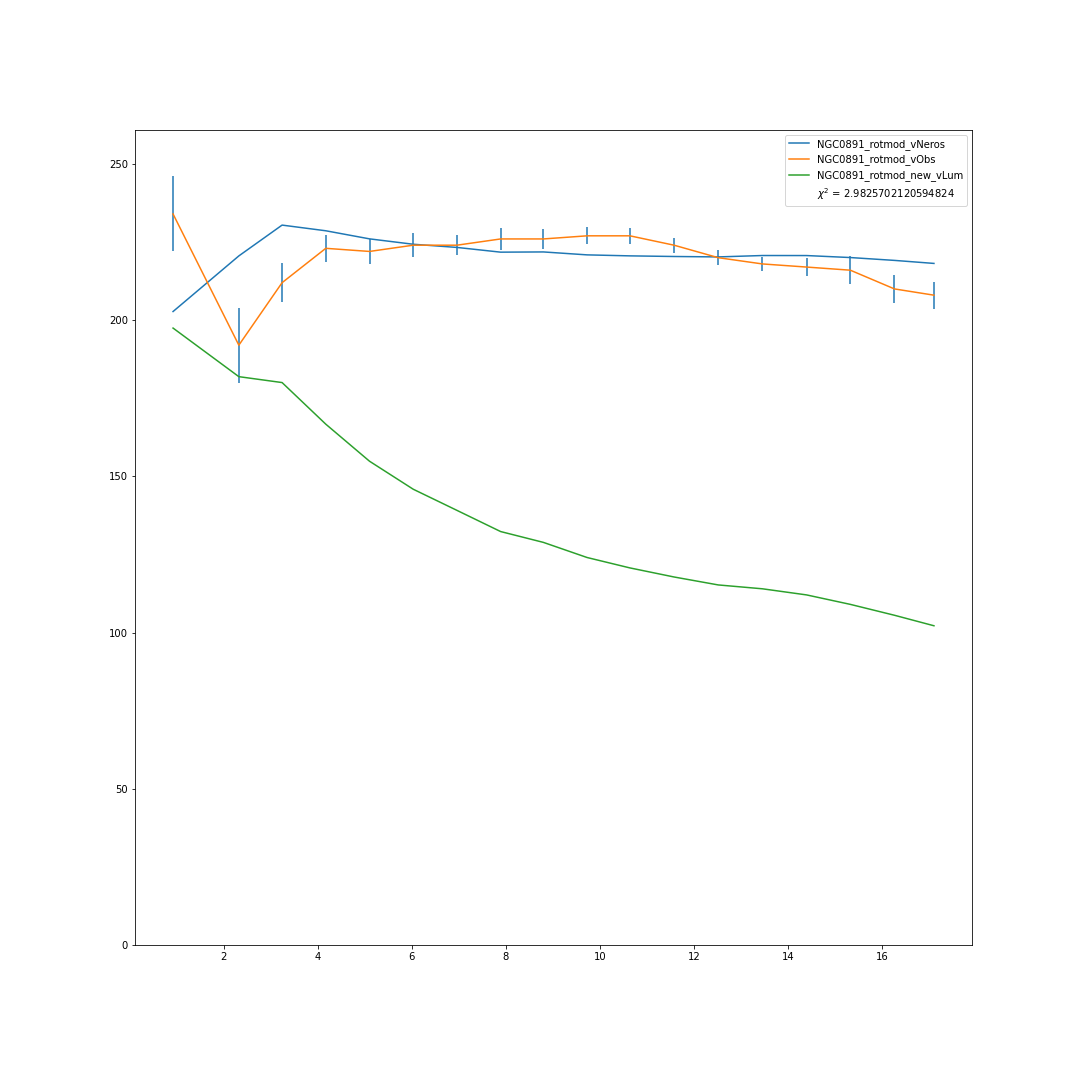
\includegraphics[width=.8\linewidth]{figures/NGC0891_rotmod_XueSofue.png}
  \caption{NGC0891}
  \label{fig:sfig12}
\end{subfigure}
\end{figure}

\clearpage
  \begin{figure}[h]
\begin{subfigure}{.5\textwidth}
  \centering
  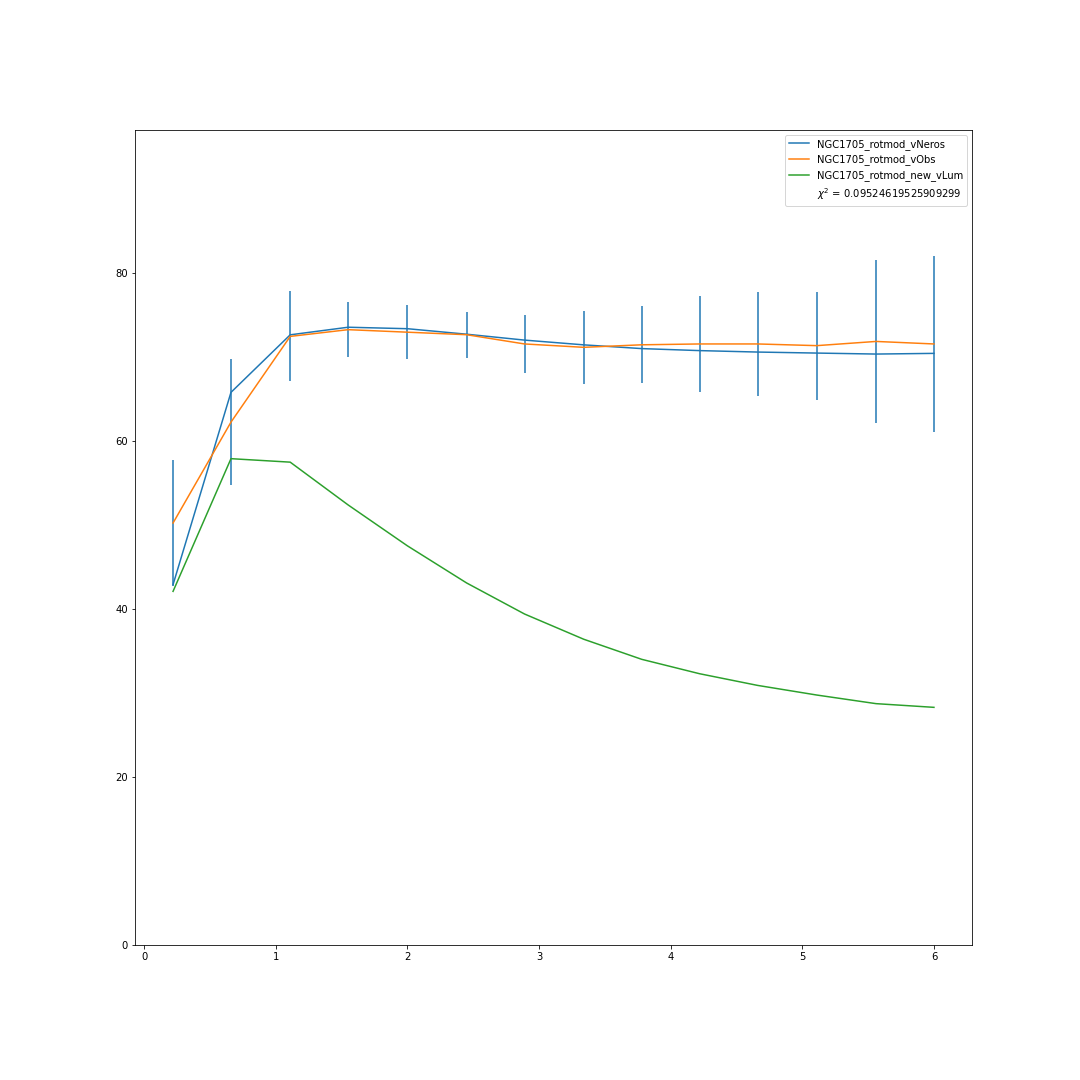
\includegraphics[width=.8\linewidth]{figures/NGC1705_rotmod_XueSofue.png}
  \caption{NGC1705}
  \label{fig:sfig13}
\end{subfigure}
\begin{subfigure}{.5\textwidth}
  \centering
  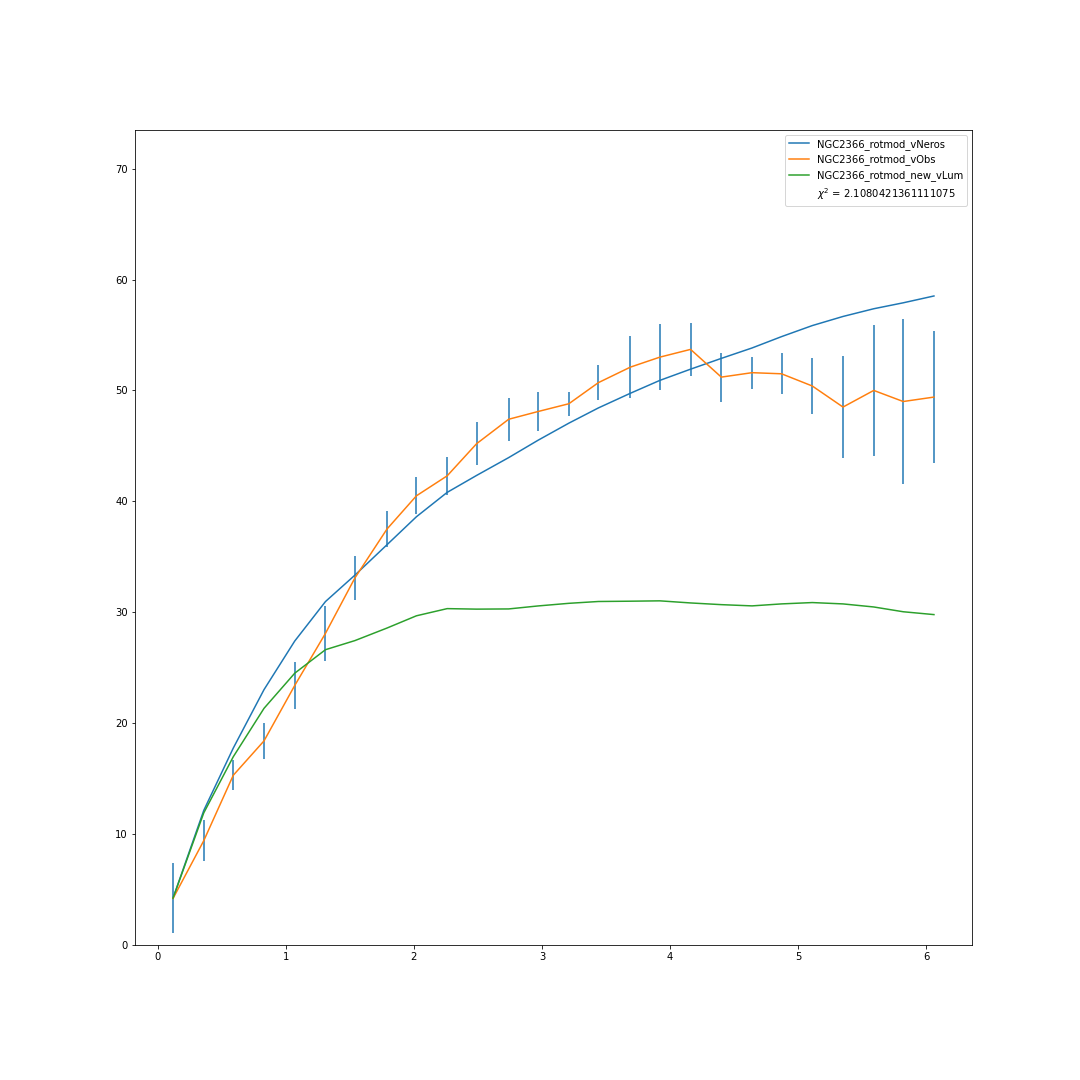
\includegraphics[width=.8\linewidth]{figures/NGC2366_rotmod_XueSofue.png}
  \caption{NGC2366}
  \label{fig:sfig14}
\end{subfigure}%
\begin{subfigure}{.5\textwidth}
  \centering
  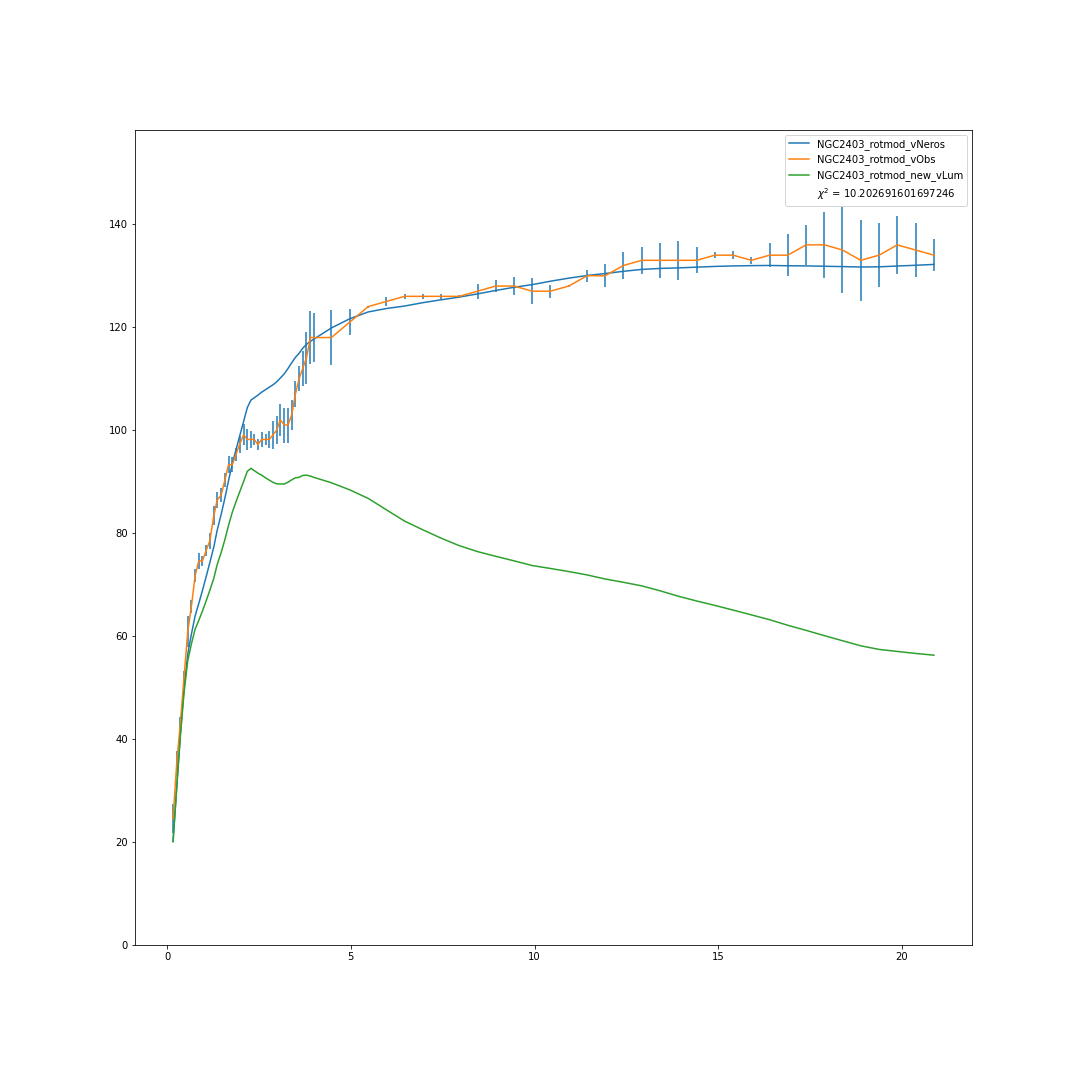
\includegraphics[width=.8\linewidth]{figures/NGC2403_rotmod_XueSofue.png}
  \caption{NGC2403}
  \label{fig:sfig15}
\end{subfigure}
\begin{subfigure}{.5\textwidth}
  \centering
  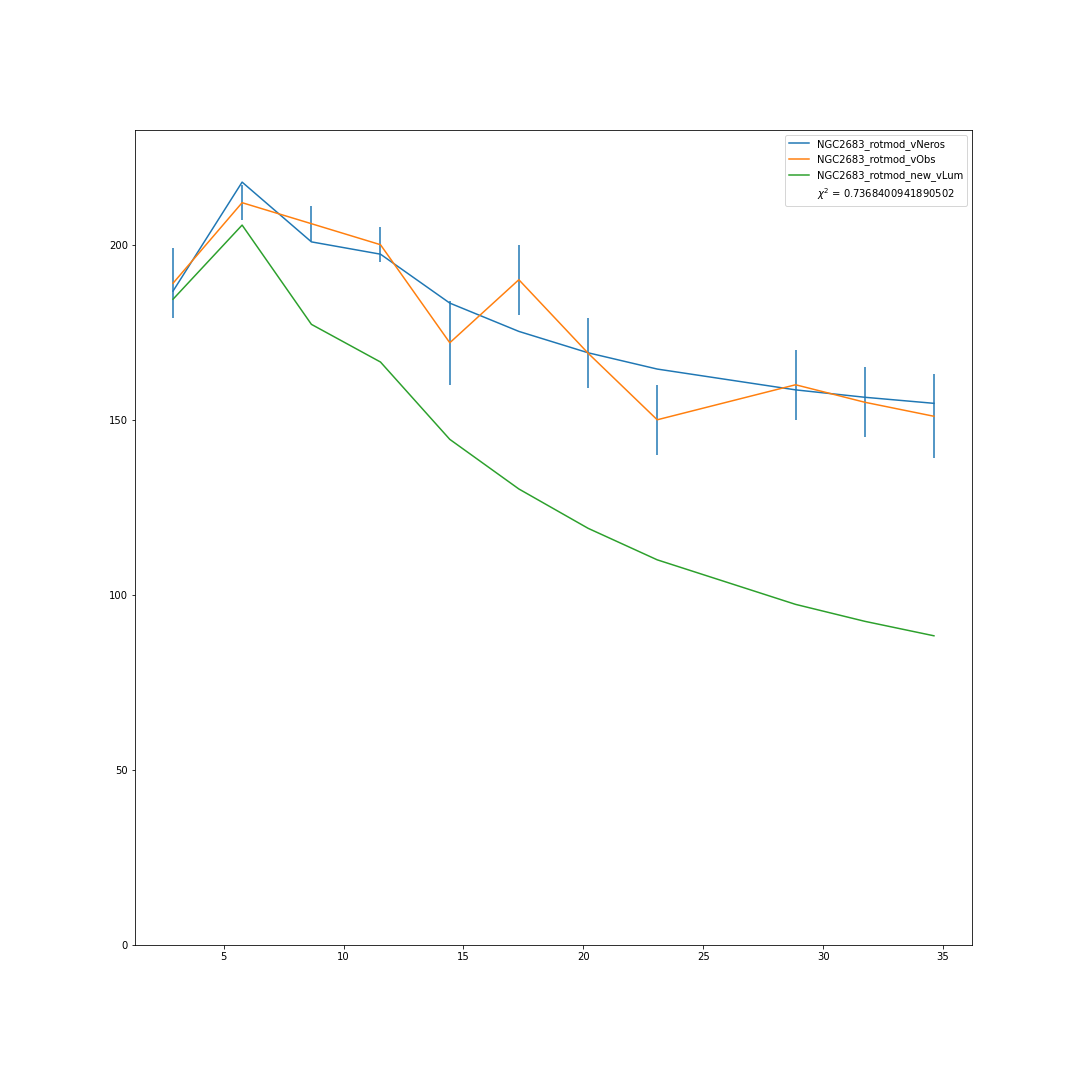
\includegraphics[width=.8\linewidth]{figures/NGC2683_rotmod_XueSofue.png}
  \caption{NGC2683}
  \label{fig:sfig16}
\end{subfigure}
\caption{ }
\label{fig:fig2903}
\end{figure}
%
\clearpage
%
%  
  \begin{figure}[h]
\begin{subfigure}{.5\textwidth}
  \centering
  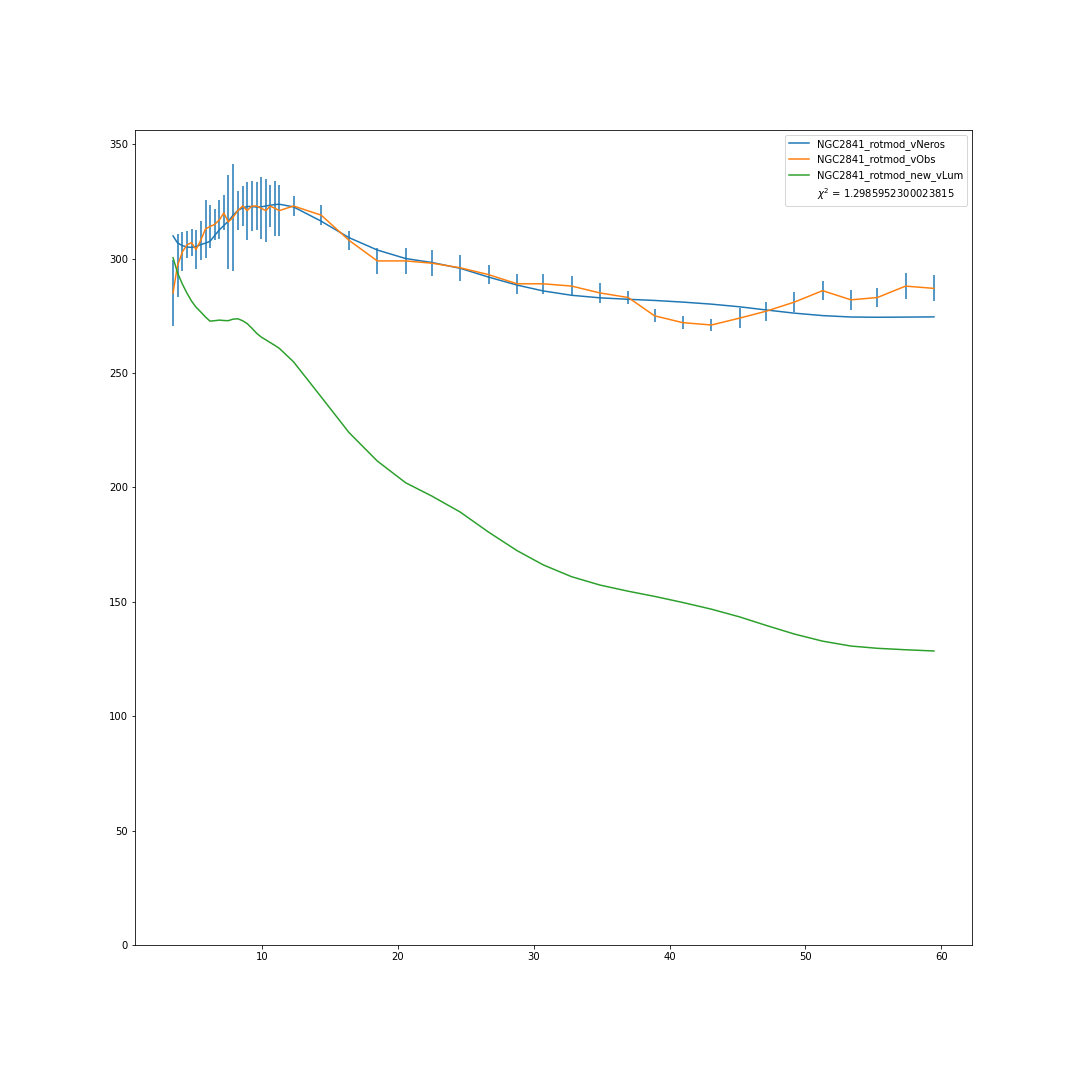
\includegraphics[width=.8\linewidth]{figures/NGC2841_rotmod_XueSofue.png}
  \caption{SPARC\cite{2016Lelli}}
  \label{fig:sfig17}
\end{subfigure}%
\begin{subfigure}{.5\textwidth}
  \centering
  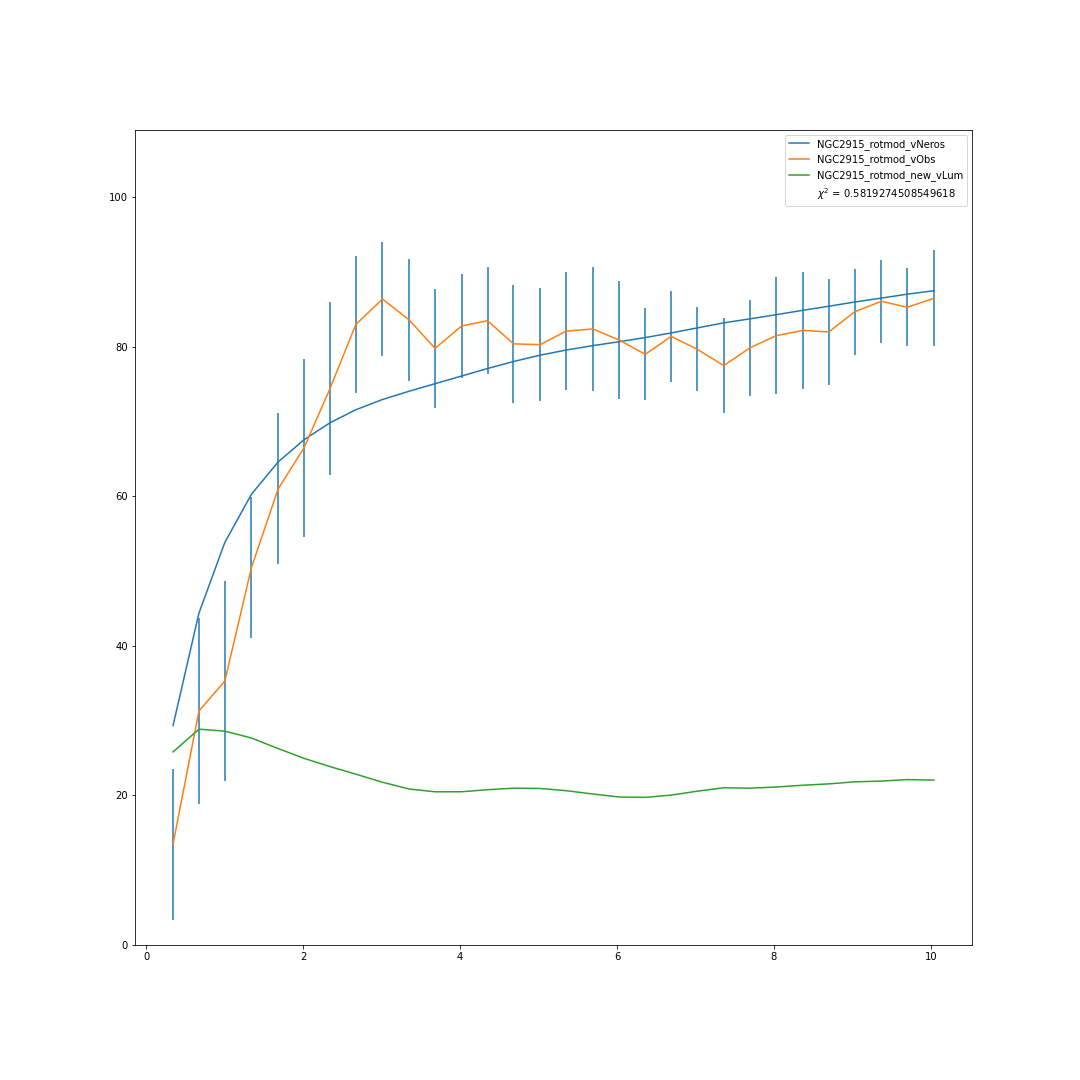
\includegraphics[width=.8\linewidth]{figures/NGC2915_rotmod_XueSofue.png}
  \caption{SPARC\cite{2016Lelli}}
  \label{fig:sfig18}
\end{subfigure}
\caption{ }
\label{fig:fig2915}
\end{figure}
%
%
%
%  
%%%%%%%
  \begin{figure}[h]
\begin{subfigure}{.5\textwidth}
  \centering
  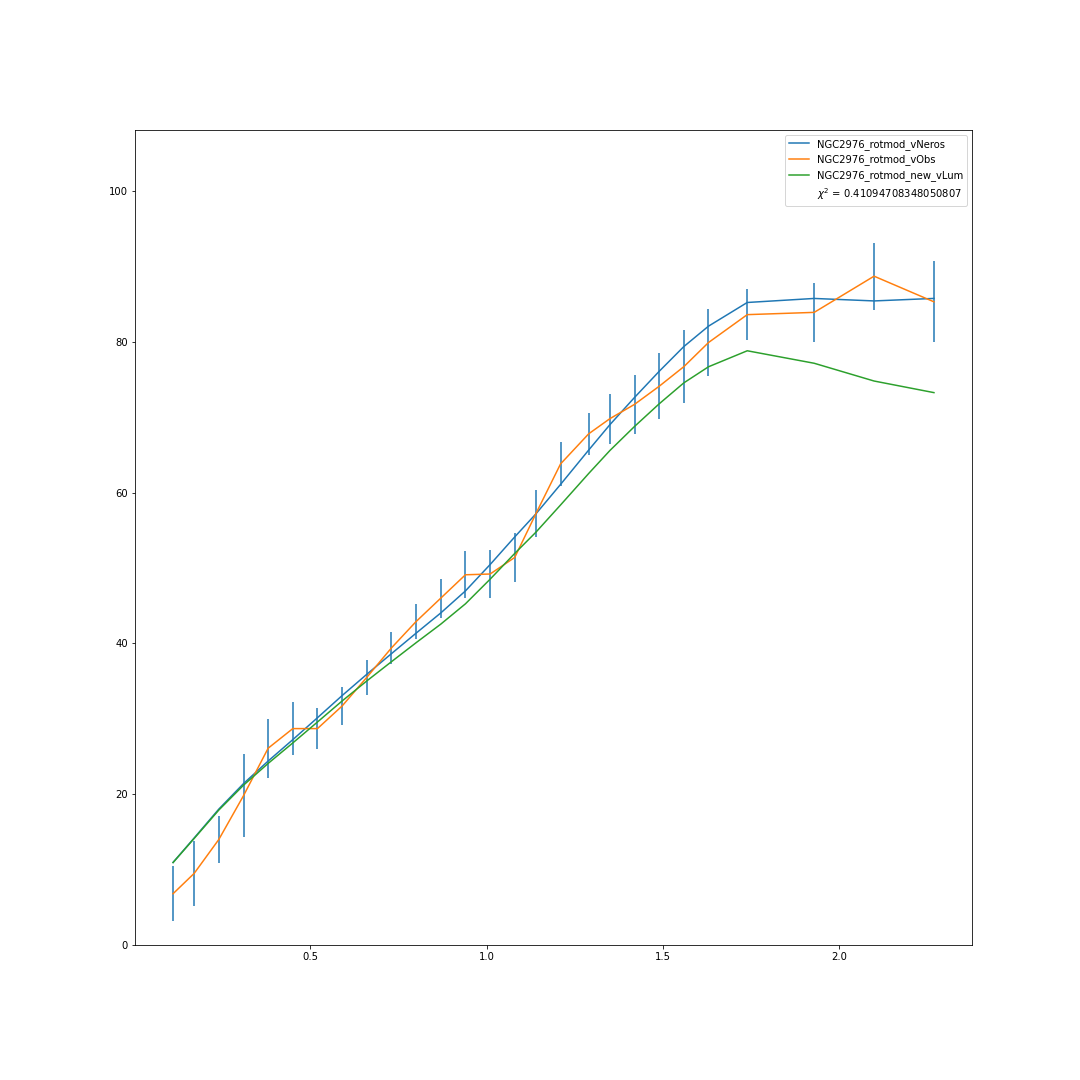
\includegraphics[width=.8\linewidth]{figures/NGC2976_rotmod_XueSofue.png}
  \caption{NGC2976}
  \label{fig:sfig19}
\end{subfigure}%
\begin{subfigure}{.5\textwidth}
  \centering
  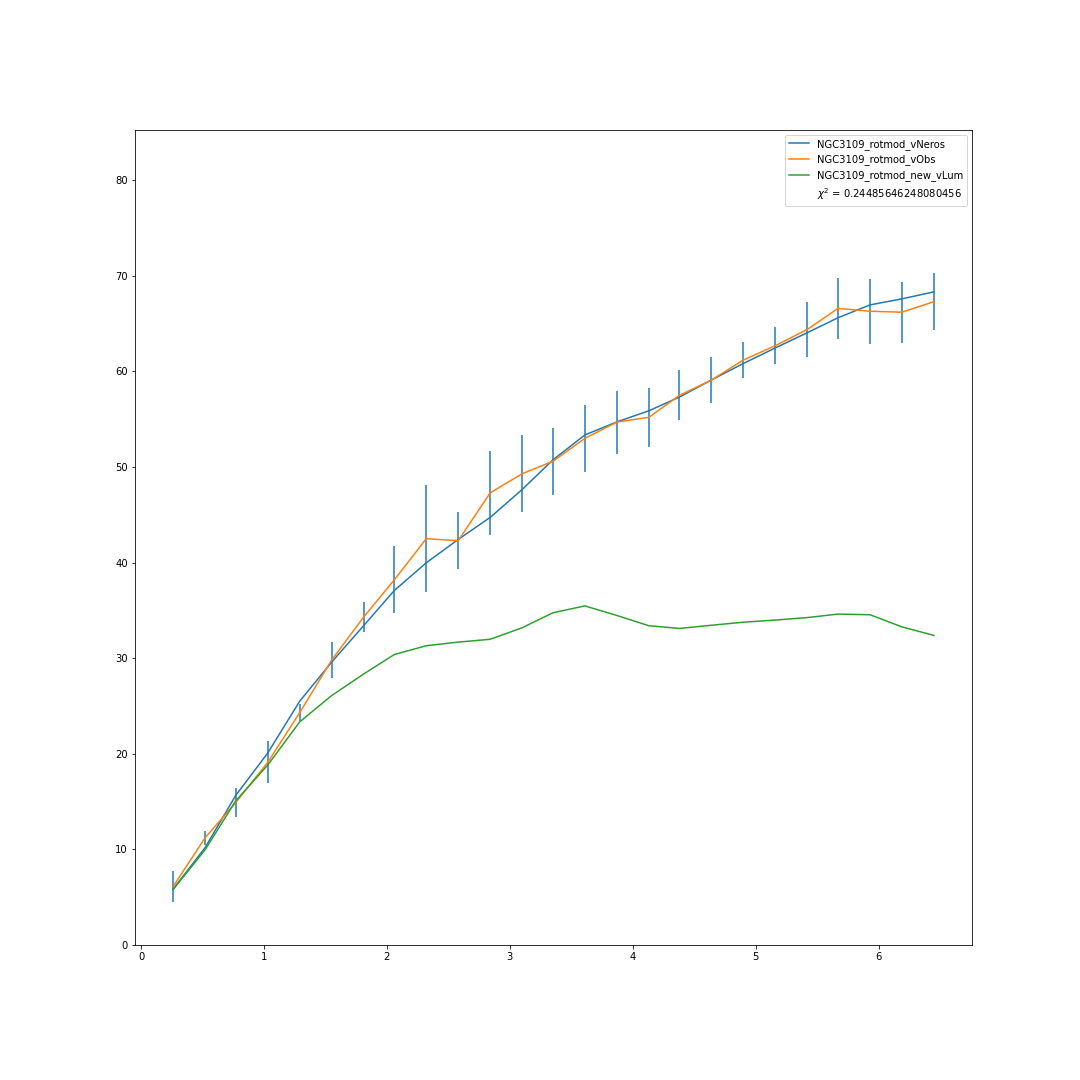
\includegraphics[width=.8\linewidth]{figures/NGC3109_rotmod_XueSofue.png}
  \caption{NGC3109}
  \label{fig:sfig20}
\end{subfigure}
\caption{ }
\label{fig:fig3521}
\end{figure}
%
%
%
\clearpage
 \begin{figure}[h]
\begin{subfigure}{.5\textwidth}
  \centering
  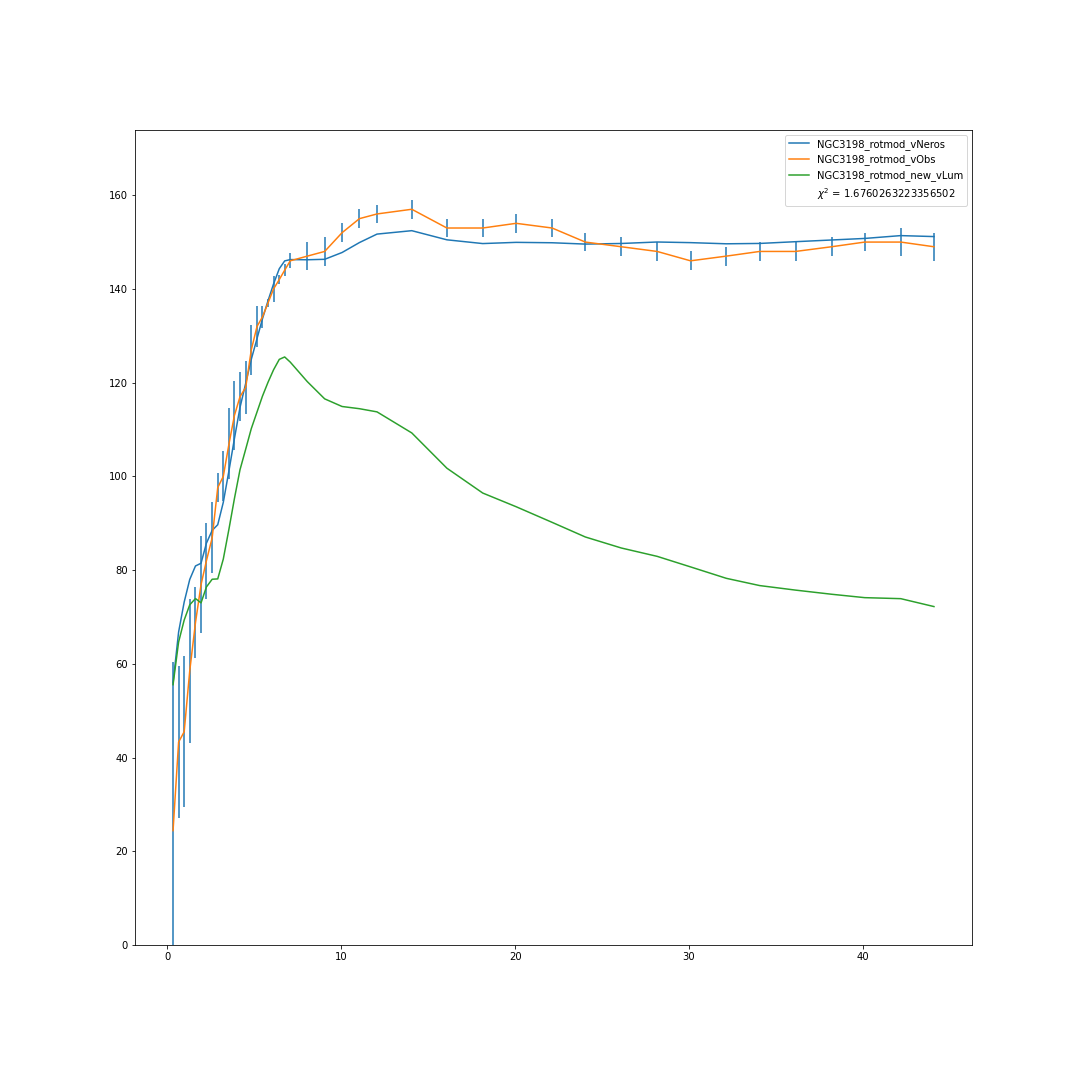
\includegraphics[width=.8\linewidth]{figures/NGC3198_rotmod_XueSofue.png}
  \caption{NGC3198}
  \label{fig:sfig21}
\end{subfigure}%
\caption{ }
\label{fig:fig7331}
\end{figure}
%%%%%%%
 
%%%%%%%%
%%%%%%
%%%%%%%
%%%%%%
  
 

    
     

\bibliography{LCM} 

\end{document}
%
% ****** End of file apssamp.tex ******